\documentclass{article}

% Language setting
\usepackage[english]{babel}

% Set page size and margins
% Replace `letterpaper' with `a4paper' for UK/EU standard size
\usepackage[a4paper,top=2cm,bottom=2cm,left=3cm,right=3cm,marginparwidth=1.75cm]{geometry}

% Useful packages
\usepackage{amsmath}
\usepackage{graphicx}
\usepackage[colorlinks=true, allcolors=blue]{hyperref}
\usepackage{lineno} % For line numbering

\title{Summary of Zucchini’s lessons}
\author{Marta Barbieri, Stefano Doria, Rossella Fioralli, Giuseppe Luciano}

\begin{document}

\maketitle
\begin{abstract}
    Ammetto che possa sembrare già incasinato ma così è strutturato in modo da essere cliccabile, le sezioni ci sono già l'unica cosa che dovete fare per iniziare il lavoro è scrivere nella regione che vi serve come nel miniesempio che sparirà. sarebbe bello fare tutto cliccabile ma solo se proprio ci annoiamo a morte da tutto il tempo che abbiamo a disposizione. se diventa troppo lungo probabilmente ci toccherà spezzettarlo però
    Regole:
    \begin{itemize}
\item \textbf{1} 
 si ha un tot di tempo dopo la lezione per aggiungere il riassunto così tutti possono studiare e non si accumula tutto alla fine. 
 
\item \textbf{2} 
Si ha l'obbligo di seguire, tranne causa di forza maggiore, la lezione da riassumere e si riassumono i pezzi spiegati nella specifica lezione seguendo le linee guida del prof 
\item \textbf{3}
Bisogna firmarsi nel capitolo riassunto così potete darmi la colpa
\item \textbf{4}
fare sempre prima un pull e poi un push sulla repository
\item \textbf{5}
altre regole?
\end{itemize}
   
\end{abstract}

\tableofcontents


%----------------------------------------------------------
\section*{1. From classical to quantum physics}

\subsection*{1.1. From classical to quantum physics}

At the end of the 19-th century, classical physics had reached a high degree of development. Newton's mechanical theory explained accurately dynamics, in particular the motion of celestial bodies. Maxwell's electromagnetic theory accounted for all electric and magnetic phenomena as well as all optical ones. Thermodynamics described the thermal properties of a broad variety of macroscopic systems with a few simple universal laws.

For a long time, mechanics was considered the ultimate physical theory providing the foundation for the other, leading in this way to the eventual unification of all physics. However, attempts to reduce electromagnetism to mechanics based on ether theory failed indicating that electromagnetism constituted an independent fundamental aspect of nature. The statistical formulation of mechanics, conversely, successfully gave a sound theoretical underpinning to thermodynamics.

Toward the end of the century, it was realized that electromagnetic waves confined in a cavity, the so called black body radiation, constitute a system much akin to a gas. All attempts to explain its thermodynamical properties by means of classical theory failed, causing a crisis of this latter that led to the birth of quantum theory.

In the several next sections, we shall give an overview of classical wave theory concentrating on such basic phenomena as interference and diffraction. Later, we shall introduce the basic notions of statistical mechanics, illustrating elementary applications.

\subsection*{1.2. Classical wave theory of light}

According to wave theory, light consists in electromagnetic waves, a form of electromagnetic field. An electromagnetic wave is described by a wave field $\psi^{1}$. This is some field characterizing the wave such as one of the components of its electric and magnetic fields or some combination of these. Technically, it is often convenient to use a complex representation of $\psi$, the real part of which furnishes the underlying physical quantity, and we shall do so in what follows.

The above approach, consisting in treating separately the single components of the electric and magnetic fields of the wave as if they were scalar fields, goes under the name of scalar wave theory. It a simple and elegant model of wave dynamics, but it is not always applicable, e. g in the analysis of polarization phenomena. When the vector nature of the wave field must be accounted for, we are referring to vector wave theory. In out treatment we shall restrict to the former and leave the latter aside.

The Maxwell equations imply that the wave field $\psi$ of light propagating in vacuum obeys the d'Alembert wave equation
 
\begin{equation*}
\nabla^{2} \psi-\frac{1}{c^{2}} \frac{\partial^{2} \psi}{\partial t^{2}}=0 \tag{1.2.1}
\end{equation*}
 
where $c$ is the speed of light in vacuum,
 
\begin{equation*}
c=2.99792458 \times 10^{10} \mathrm{~cm} \mathrm{sec}^{-1} \tag{1.2.2}
\end{equation*}
 

Light produced by distinct sources in the same spacial region can and does blend. In wave theory, this experimentally revealed fact is reflected in the superposition principle: two or more electromagnetic waves can propagate simulta-

\footnotetext{
${ }^{1}$ Recall that a field is any quantity $f(t, \boldsymbol{x})$ whose value depends on the observation time $t$ and place $\boldsymbol{x}$.
}

![](https://cdn.mathpix.com/cropped/2024_09_22_5d1e855547710648961eg-0015.jpg?height=839&width=1074&top_left_y=502&top_left_x=471)

Figure 1.2.1. The wave $(c)$ is the superposition of the waves $(a)$ and $(b)$ with weight $1 / 2$ each. The dashed brown line represents schematically space. The superposition is taken at a fixed time.
neously in a region generating together another electromagnetic wave, which is their superposition. This possibility rests on a basic property of the wave equation (1.2.1), its linearity: if $\psi_{k}$ is a collection of solutions of (1.2.1) and $c_{k}$ are complex constants, then the linear combination
 
\begin{equation*}
\psi=\sum_{k} c_{k} \psi_{k} \tag{1.2.3}
\end{equation*}
 
is also a solution of (1.2.1). More generally, if $\psi_{\varkappa}$ is a family of solutions of (1.2.1) parametrized by one or more continuous variables collectively denoted by $\varkappa$ and $c_{\varkappa}$ are complex functions of the $\varkappa$, then the linear combination
 
\begin{equation*}
\psi=\int d \varkappa c_{\varkappa} \psi_{\varkappa} \tag{1.2.4}
\end{equation*}
 
is also a solution of (1.2.1). See fig. 1.2.1 for a pictorial illustration of superposition of waves.

The superposition principle makes it possible to express a generic wave as a superposition of monochromatic waves, to which we now turn.

\subsection*{1.3. Monochromatic waves}

In classical wave theory, monochromatic light is composed by monochromatic waves. A wave is said monochromatic, if its associated wave field $\psi_{t}$ has a sinusoidal time dependence of the form
 
\begin{equation*}
\psi_{t}=\psi_{0} \exp (-i \omega t) \tag{1.3.1}
\end{equation*}
 
where we make explicit the time dependence of a generic field $f$ by treating it as time dependent spacial field $f_{t}$ with $f_{t}(\boldsymbol{x})=f(t, \boldsymbol{x})$. The constant $\omega$ has the dimension of an inverse time and is called angular frequency. The $t=0$ wave field $\psi_{0}$ satisfies a simplified version of the d'Alembert wave equation (1.2.1), the Helmholtz wave equation,
 
\begin{equation*}
\nabla^{2} \psi_{0}+\kappa^{2} \psi_{0}=0 \tag{1.3.2}
\end{equation*}
 
where $\kappa$ is a constant with the dimension of an inverse length given by
 
\begin{equation*}
\kappa=\omega / c \tag{1.3.3}
\end{equation*}
 
and called angular wave number.

![](https://cdn.mathpix.com/cropped/2024_09_22_5d1e855547710648961eg-0017.jpg?height=451&width=993&top_left_y=1935&top_left_x=555)

Figure 1.3.1. A monochromatic wave has a sinosoidal time dependence.

Proof. Substituting (1.3.1) into (1.2.1), we get
 
\begin{align*}
0=\nabla^{2} \psi_{t}-\frac{1}{c^{2}} \frac{\partial^{2} \psi_{t}}{\partial t^{2}}=\nabla^{2} \psi_{0} \exp (-i \omega t) & -\psi_{0} \frac{1}{c^{2}} \frac{\partial^{2}}{\partial t^{2}} \exp (-i \omega t)  \tag{1.3.4}\\
& =\left(\nabla^{2} \psi_{0}+\frac{\omega^{2}}{c^{2}} \psi_{0}\right) \exp (-i \omega t)
\end{align*}
 
obtaining (1.3.2).

A monochromatic wave is characterized by two more parameters, the period $\tau$ and wavelength $\lambda$ defined by
 
\begin{equation*}
\tau=2 \pi / \omega, \quad \lambda=2 \pi / \kappa \tag{1.3.5}
\end{equation*}
 
with the dimension of a time and a length, respectively, and related as
 
\begin{equation*}
\lambda=c \tau \tag{1.3.6}
\end{equation*}
 
$\tau$ is the period of $\psi_{t}$ as a sinusoidal function of $t . \lambda$ is the distance $\psi_{t}$ propagates in a time $\tau$. This leads us to the study of wave propagation.

The complex wave field $\psi_{t}$ can be decomposed in two real fields, the phase $\varphi_{t}$ and the amplitude $a_{t}$, defined by the relation
 
\begin{equation*}
\psi_{t}=a_{t} \exp \left(i \varphi_{t}\right) \tag{1.3.7}
\end{equation*}
 

The amplitude-phase decomposition is very natural from a physical point of view, since it answers to the intuitive picture of a wave. Indeed, the phase $\varphi$ and the the amplitude $a$ of the wave describe the propagation and the intensity of the light associated with the wave.

On account of (1.3.1), the time dependence of $\varphi_{t}, a_{t}$ has the simple form
 
\begin{align*}
\varphi_{t} & =\varphi_{0}-\omega t  \tag{1.3.8}\\
a_{t} & =a_{0} \tag{1.3.9}
\end{align*}
 

Proof. Indeed, by (1.3.1), we have using (1.3.7)
 
\begin{align*}
a_{t} \exp \left(i \varphi_{t}\right)=\psi_{t}= & \psi_{0} \exp (-i \omega t)  \tag{1.3.10}\\
& =a_{0} \exp \left(i \varphi_{0}\right) \exp (-i \omega t)=a_{0} \exp \left(i\left(\varphi_{0}-\omega t\right)\right)
\end{align*}
 
(1.3.8), (1.3.9) follow.

A wave front of a wave is the locus of the points of space having a fixed phase, that is the set of the points $\boldsymbol{x}$ satisfying an equation of the form
 
\begin{equation*}
\varphi_{t}(\boldsymbol{x})=\alpha \tag{1.3.11}
\end{equation*}
 
where $\alpha$ is a fixed constant angle. By (1.3.8), (1.3.11) can be written as
 
\begin{equation*}
\varphi_{0}(\boldsymbol{x})=\omega t+\alpha \tag{1.3.12}
\end{equation*}
 

Geometrically, so, the wave front is a surface $\mathcal{S}_{t}$ depending on the time $t$. As $t$ elapses, the location of $\mathcal{S}_{t}$ shifts in space leading to the wave's propagation (cf. fig. 1.3.2). At any time $t$, the location of $\mathcal{S}_{t}$ coincides with precisely one member of the one parameter family of surfaces $\mathcal{S}_{\sigma}$ defined by $\varphi_{0}(\boldsymbol{x})=\sigma$ which foliate space. Since every point $\boldsymbol{x}$ lies in precisely one surface $\mathcal{S}_{\sigma}$, the wave front passing for a given point $\boldsymbol{x}$ at any time $t$ is independent from $t$ as a geometrical point set. A ray is any line in space such that the unit vector tangent at each point $\boldsymbol{x}$ of the line in normal to the surface $\mathcal{S}_{\sigma}$ passing through $\boldsymbol{x}$.

The phase velocity $v$ of a wave at the certain point is the velocity at which a wave front passing instantaneously at that point propagates. It is given by
 
\begin{equation*}
v=\frac{\omega}{\left|\boldsymbol{\nabla} \varphi_{0}\right|} \tag{1.3.13}
\end{equation*}
 

Note that it may differ and even exceed the light speed $c$.

Proof. If $\boldsymbol{y}$ is a vector tangent to $\mathcal{S}_{t}$ at a point $\boldsymbol{x}$, there exists a parametrized curve $\boldsymbol{\xi}(s)$ entirely contained in $\mathcal{S}_{t}$ with the property that $\boldsymbol{\xi}(0)=\boldsymbol{x}$ and $d \boldsymbol{\xi}(0) / d s=\boldsymbol{y}$. Since
$\varphi_{0}(\boldsymbol{\xi}(s))-\varphi_{0}(\boldsymbol{x})=0$ identically by (1.3.12), we have
 
\begin{equation*}
0=\left.\frac{d}{d s}\left(\varphi_{0}(\boldsymbol{\xi}(s))-\varphi_{0}(\boldsymbol{x})\right)\right|_{s=0}=\frac{d \boldsymbol{\xi}(0)}{d s} \cdot \boldsymbol{\nabla} \varphi_{0}(\boldsymbol{\xi}(0))=\boldsymbol{y} \cdot \boldsymbol{\nabla} \varphi_{0}(\boldsymbol{x}) \tag{1.3.14}
\end{equation*}
 

Thus, the normal unit vector to $\mathcal{S}_{t}$ at $\boldsymbol{x}$ is
 
\begin{equation*}
\boldsymbol{n}(\boldsymbol{x})=\frac{\boldsymbol{\nabla} \varphi_{0}(\boldsymbol{x})}{\left|\boldsymbol{\nabla} \varphi_{0}(\boldsymbol{x})\right|} \tag{1.3.15}
\end{equation*}
 

In the time interval from $t$ to $t+\Delta t$, the vave front $\mathcal{S}_{t}$ sweeps a given ray from a point $\boldsymbol{x}$ to a point $\boldsymbol{x}+\Delta \boldsymbol{x}$ on the ray. As the ray is normal at each of its points to the wave front through that point, the front advances in the normal direction a distance
 
\begin{equation*}
\Delta d=\boldsymbol{n}(\boldsymbol{x}) \cdot \Delta x \tag{1.3.16}
\end{equation*}
 

The speed of the front is therefore
 
\begin{equation*}
v(\boldsymbol{x})=\frac{\Delta d}{\Delta t}=\boldsymbol{n}(\boldsymbol{x}) \cdot \frac{\Delta \boldsymbol{x}}{\Delta t}=\frac{\boldsymbol{\nabla} \varphi_{0}(\boldsymbol{x})}{\left|\boldsymbol{\nabla} \varphi_{0}(\boldsymbol{x})\right|} \cdot \frac{\Delta \boldsymbol{x}}{\Delta t} \tag{1.3.17}
\end{equation*}
 

Since (1.3.12) must hold identically during the propagation of the wave front, we have $\varphi_{0}(\boldsymbol{x}+\Delta \boldsymbol{x})-\omega(t+\Delta t)=\varphi_{0}(\boldsymbol{x})-\omega t$. So, by Taylor's formula, $\Delta t$ and $\Delta \boldsymbol{x}$ obey
 
\begin{equation*}
\boldsymbol{\nabla} \varphi_{0}(\boldsymbol{x}) \cdot \Delta \boldsymbol{x}-\omega \Delta t=0 \tag{1.3.18}
\end{equation*}
 

Figure 1.3.2. A typical pattern of wave fronts (brown) and rays (yellow).

Using (1.3.18) in (1.3.17), we get
 
\begin{equation*}
v(\boldsymbol{x})=\frac{\omega}{\left|\boldsymbol{\nabla} \varphi_{0}(\boldsymbol{x})\right|} \tag{1.3.19}
\end{equation*}
 
(1.3.13) is so shown.

Monochromatic waves can be classified according to the geometrical shape of their wave fronts. In particular, they can be plane, spherical, cylindrical, etc. Once the shape of the wave front is assigned, the wave equation (1.3.2) determine the analytic form of the wave field.

The wave field $\psi$ of a plane monochromatic wave has the form
 
\begin{equation*}
\psi(t, \boldsymbol{x})=u_{0} \exp (i(\kappa z-\omega t)) \tag{1.3.20}
\end{equation*}
 
where $z=\boldsymbol{n} \cdot \boldsymbol{x}$ is the height of the observation point $\boldsymbol{x}$ from the plane through $\mathbf{0}$ normal to the unit vector $\boldsymbol{n}$ and $u_{0}$ is a complex constant. The wave number $\kappa$ and $\boldsymbol{n}$ are naturally combined in the wave vector
 
\begin{equation*}
\boldsymbol{\kappa}=\kappa \boldsymbol{n} \tag{1.3.21}
\end{equation*}
 

![](https://cdn.mathpix.com/cropped/2024_09_22_5d1e855547710648961eg-0021.jpg?height=700&width=912&top_left_y=1699&top_left_x=585)

Figure 1.3.3. The wave front pattern of a plane wave.
$\boldsymbol{\kappa}$ fully characterizes the wave. The wave fronts are the planes normal to $\boldsymbol{n}$ defined by the equation $\kappa z-\omega t=\alpha$ (cf. fig. 1.3.3). As time flows, these planes shifts in the direction of $\boldsymbol{n}$ with phase speed $\omega / \kappa=c$. The wave's rays are straight lines parallel to $\boldsymbol{n}$.

The wave field of a spherical monochromatic wave has the form
 
\begin{equation*}
\psi(t, \boldsymbol{x})=u_{0} \frac{\exp (i( \pm \kappa r-\omega t))}{r} \tag{1.3.22}
\end{equation*}
 
where $r=|\boldsymbol{x}|$ is the distance of the observation point $\boldsymbol{x}$ from the origin $\mathbf{0}$ and $u_{0}$ is a complex constant. The wave fronts of such a wave are the spheres centered in $\mathbf{0}$ defined by $\pm \kappa r-\omega t=\alpha$ (cf. fig. 1.3.4). As time flows, these spheres expand from or shrink to $\mathbf{0}$ at phase speed $\omega / \kappa=c$ according to whether the sign is $+/-$. The wave's rays are straight half lines emanating from $\mathbf{0}$.

The wave field of a cylindrical monochromatic wave has the asymptotic form
 
\begin{equation*}
\psi(t, \boldsymbol{x})=u_{0} \frac{\exp (i( \pm \kappa r-\omega t))}{r^{1 / 2}}, \quad \kappa r \gg 1 \tag{1.3.23}
\end{equation*}
 
where $r=|\boldsymbol{x}-\boldsymbol{x} \cdot \boldsymbol{n} \boldsymbol{n}|$ is the distance of the observation point $\boldsymbol{x}$ from the axis through the origin $\mathbf{0}$ oriented along the unit vector $\boldsymbol{n}$ and $u_{0}$ is a complex

![](https://cdn.mathpix.com/cropped/2024_09_22_5d1e855547710648961eg-0022.jpg?height=621&width=619&top_left_y=1755&top_left_x=729)

Figure 1.3.4. The wave front pattern of a spherical wave.

![](https://cdn.mathpix.com/cropped/2024_09_22_5d1e855547710648961eg-0023.jpg?height=597&width=720&top_left_y=550&top_left_x=735)

Figure 1.3.5. The wave front pattern of a cylindrical wave.
constant. The above expression, although analogous to that of a spherical wave, differs from this latter in that it holds anly for large radius $r$. The wave fronts of such a wave are the cylinders with axis $\boldsymbol{n}$ defined by $\pm \kappa r-\omega t=\alpha$ (cf. fig. 1.3.5). As time flows, these cylinders expand from or contract to the axis at phase speed $\omega / \kappa=c$ according to whether the sign is $+/-$. The wave's rays are straight half lines emanating from the axis perpendicularly to it.

Remark. A source of electromagnetic waves emits waves in trains. The time at which the emission process of a train begins, that at which it ends and the duration of the emission are normally completely random. Therefore, even if the source emits with a well defined frequency $\omega$, the waves it produces are not quite monochromatic. Their wavefield $\psi_{t}$ has still the phase-amplitude decomposition (1.3.7), but the time dependence of the phase $\varphi_{t}$ is not of the simple form (1.3.8), but rather
 
\begin{equation*}
\varphi_{t}=\varphi_{0}-\omega t+\alpha(t) \tag{1.3.24}
\end{equation*}
 
where $\alpha(t)$ is a function of time that is constant over a certain time $\Delta t$ but suffers completely random discontinuities over a time much larger than $\Delta t$. One calls $\Delta t$ the coherence time of the wave. It is typically large with respect to the period $\tau$ but finite.

The larger $\Delta t$, the more coherent the wave is. A monochromatic wave is an ideal wave having an infinite coherence time and, so, a completely coherent one.

\subsection*{1.4. Wave propagation and Huygens' principle}

The propagation in space of a wave front $\mathcal{S}_{t}$ of a monochromatic wave of frequency $\omega$ as $t$ flows is described by the Huygens' principle.

Each point $\boldsymbol{\xi}$ of the wave front $\mathcal{S}_{t}$ at time $t$ acts as a point source of an outgoing spherical monochromatic wave of frequency $\omega$. The wave front $\mathcal{S}_{t^{\prime}}$ at time $t^{\prime}>t$ is the envelope enclosing the wave fronts $\mathcal{S}_{\xi t^{\prime}}$ of the spherical waves emanating from all points $\boldsymbol{\xi}$ of $\mathcal{S}_{t}$, that is the surface that at each of its points $\boldsymbol{\xi}^{\prime}$ is tangent to the wave front $\mathcal{S}_{\xi t^{\prime}}$ passing through $\boldsymbol{\xi}^{\prime}$.

The principle is illustrated pictorially in fig. 1.4.1.
The Huygens principle can be rephrased as a particular case of the superposition principle (cf. sect. 1.2). At any time $t^{\prime}$, the wave field $\psi_{t^{\prime}}$ of the primary wave is the superposition of the wave fields $\psi_{\xi t^{\prime}}$ of the secondary spherical waves,
 
\begin{equation*}
\psi_{t^{\prime}}=\int_{\mathcal{S}_{t}} d^{2} \xi \psi_{\xi t^{\prime}} \tag{1.4.1}
\end{equation*}
 

As the secondary waves are monochromatic spherical ones of frequency $\omega, \psi_{\boldsymbol{\xi} t}$ is explicitly given by (1.3.22),
 
\begin{equation*}
\psi_{\boldsymbol{\xi}}(t, \boldsymbol{x})=w_{\boldsymbol{\xi}} \frac{\exp \left(i\left(\kappa r_{\boldsymbol{\xi}}-\omega t\right)\right)}{r_{\boldsymbol{\xi}}} \tag{1.4.2}
\end{equation*}
 
where $r_{\boldsymbol{\xi}}=|\boldsymbol{x}-\boldsymbol{\xi}|$ is the distance of the observation point $\boldsymbol{x}$ from center $\boldsymbol{\xi}$ of the wave, $\kappa$ is the wave number given by (1.3.3) and $w_{\xi}$ is a complex constant. The

![](https://cdn.mathpix.com/cropped/2024_09_22_5d1e855547710648961eg-0025.jpg?height=280&width=1034&top_left_y=2099&top_left_x=513)

Figure 1.4.1. Schematic geometrical representation of Huygens' principle.
phase of $w_{\boldsymbol{\xi}}$ is independent from $\boldsymbol{\xi}$, as the secondary waves all originate from the same wave front at the same time $t$ and, so, they must have the same phase at their respective origins.

Remark. The expression (1.4.1) calculating the wave field of a propagating wave is defective in the following respect. The spherical waves $\mathcal{S}_{\xi t^{\prime}}$ departing form the wave front $\mathcal{S}_{t}$ generate through their envelope the wave front $\mathcal{S}_{t^{\prime}}$ only in the forward direction, but not in the backward one. It is thus necessary to insert in the integrand of (1.4.1) an inclination factor $K$ varying smoothly from the value 1 to 0 when passing from the positive normal direction to the wave front $\mathcal{S}_{t}$ to the negative one.

\subsection*{1.5. Light interference}

Interference may be described as the process whereby the monochromatic light radiated by two or more sources under certain conditions produces a pattern of bright and dark patches on a screen. Interference is an optical phenomenon that shows the undulatory nature of light quite distinctly and is indeed described accurately by classical wave theory.

As the light's brightness or dimness is measured by the light's intensity, interference involves a modulation of this latter. In wave theory, intensity is directly related to the flux of electromagnetic energy of the associated electromagnetic waves. More specifically, the intensity $I$ is the amount of electromagnetic energy flowing per unit time through the unit area transverse to the flow direction. For monochromatic waves, to which we shall restrict, the energy flux is proportional to the square magnitude of the electric or magnetic fields. $I$, consequently, is proportional to the square magnitude of the wave field $\psi$. We thus have
 
\begin{equation*}
I=g_{0}\left|\psi_{0}\right|^{2} \tag{1.5.1}
\end{equation*}
 
where $g_{0}$ is a constant. In the right hand side, we have taken $\psi_{t}$ at time $t=0$ since, being the wave monochromatic, $\psi_{t}$ is of the form (1.3.1) and, so, $\left|\psi_{t}\right|^{2}$ does not depend on $t$. I is so time independent. But, as $\psi_{0}$ is a field, $I$ is position dependent. By (1.3.7), $I$ is expressible also in terms of the amplitude $a_{0}$ of $\psi_{0}$ as
 
\begin{equation*}
I=g_{0} a_{0}{ }^{2} \tag{1.5.2}
\end{equation*}
 

Suppose that a set of sources emit waves of wave field $\psi_{j}$ and intensity $I_{j}$. Upon superposition, a wave of wave field $\psi$ and intensity $I$ is produced. The components contribute to the superposition with an equal weight, which we may take to be 1 . From (1.2.3), therefore, $\psi_{t}$ is given by
 
\begin{equation*}
\psi_{t}=\sum_{j} \psi_{j t} \tag{1.5.3}
\end{equation*}
 

One finds then that the intensities $I_{j}$ and $I$ are related as
 
\begin{equation*}
I=\sum_{j} I_{j}+2 \sum_{j<k}\left(I_{j} I_{k}\right)^{1 / 2} \cos \varphi_{j k 0} \tag{1.5.4}
\end{equation*}
 
where $\varphi_{j k 0}=\varphi_{j 0}-\varphi_{k 0}, \varphi_{j 0}$ being the phase of $\psi_{j 0}$ defined according to (1.3.7).

Proof. Inserting (1.5.3) into expression (1.5.1) and exploiting the algebraic identity $\left|\Sigma_{j} z_{j}\right|^{2}=\Sigma_{j}\left|z_{j}\right|^{2}+2 \Sigma_{j<k} \operatorname{Re}\left(z_{j}{ }^{*} z_{k}\right)$, we find
 
\begin{align*}
I=g_{0}\left|\psi_{0}\right|^{2}=g_{0} \sum_{j}\left|\psi_{j 0}\right|^{2}+2 g_{0} \sum_{j<k}\left|\psi_{j 0}\right|\left|\psi_{k 0}\right| & \operatorname{Re}\left(\frac{\psi_{j 0}{ }^{*} \psi_{k 0}}{\left|\psi_{j 0}\right|\left|\psi_{k 0}\right|}\right)  \tag{1.5.5}\\
& =\sum_{j} I_{j}+2 \sum_{j<k}\left(I_{j} I_{k}\right)^{1 / 2} \gamma_{j k 0}
\end{align*}
 
where the $\gamma_{j k}$ are given by
 
\begin{equation*}
\gamma_{j k 0}=\operatorname{Re}\left(\frac{\psi_{j 0}{ }^{*} \psi_{k 0}}{\left|\psi_{j 0}\right|\left|\psi_{k 0}\right|}\right) \tag{1.5.6}
\end{equation*}
 

Expressing each wave field $\psi_{l 0}$ in terms of its phase $\varphi_{l 0}$ and amplitude $a_{l 0}$ as in (1.3.7) in (1.5.6), we obtain so
 
\begin{equation*}
\gamma_{j k 0}=\operatorname{Re}\left(\exp \left(-i \varphi_{j 0}+i \varphi_{k 0}\right)\right)=\cos \varphi_{j k 0} \tag{1.5.7}
\end{equation*}
 

Substituting (1.5.7) into (1.5.5), we obtain (1.5.4).

Normally, the phase $\varphi_{j 0}$ of $\psi_{j 0}$ is a much more sensitive function of position than the amplitude $a_{j 0}$ of $\psi_{j 0}$ is. Thus, the intensities $I_{j}=g_{0} a_{j 0}{ }^{2}$ are slowly varying functions of the observation point while the cosines $\cos \varphi_{j k 0}$ are rapidly varying ones. Because of the second term in the right hand side of (1.5.4), so, $I$, as a function of the observation point, can take values both markedly greater and smaller than $\sum_{j} I_{j}$ in any spacial region where this latter is approximately constant. $I$ exhibits in this way a series of maxima and minima. In the former case, we have constructive, in the latter destructive interference.

Remark. In the above analysis, we have assumed that the waves involved in interference are are rigorously monochromatic and, thus, completely coherent (see the
remark at the end of sect. 1.3). In real interference experiments, instead, the waves dealt with are only approximately monochromatic and, consequently, only partially coherent. Their phases $\varphi_{j t}$ have thus the form
 
\begin{equation*}
\varphi_{j t}=\varphi_{j 0}-\omega t+\alpha_{j}(t) \tag{1.5.8}
\end{equation*}
 
where $\alpha_{j}(t)$ is a function of time that is constant over the coherence time $\Delta t$ but suffers completely random discontinuities over a time much larger than $\Delta t$ (cf. eq. 1.3.24). If we now repeat our calculations in this more realistic situation with the wave fields $\psi_{j t}$ evaluated at the observation time $t$, we find that the intensity of the $j$-th component is still $I_{j}=g_{0} a_{j 0}{ }^{2}$, while the intensity of the superposition becomes
 
\begin{equation*}
I_{t}=\sum_{j} I_{j}+2 \sum_{j<k}\left(I_{j} I_{k}\right)^{1 / 2} \cos \varphi_{j k t} \tag{1.5.9}
\end{equation*}
 
where $\varphi_{j k t}=\varphi_{j t}-\varphi_{k t}=\varphi_{j k 0}+\alpha_{j}(t)-\alpha_{k}(t) \cdot \cos \varphi_{j k t}$ varies rapidly and unpredictably as the time $t$ flows. The measurement of intensity requires a time much longer than the typical time scale of such rough variations. Thus, only the time average of the second term is actually detected. But this average vanishes identically because of the random nature of the time dependence of the $\alpha_{j}(t)$ unless $\alpha_{j}(t)=\alpha(t)$ independent from $j$. When this happens, the waves are said reciprocally coherent. Interference is then observed only when the waves have this property. Reciprocally coherent waves are produced only in special situations. Waves produced by division of the wave front of an approximately monochromatic wave are obviously coherent, since the time dependent part of their phases has the form $-\omega t+\alpha(t)$ with $\alpha(t)$ a random phase for all of them.

Remark. The mechanism of wave propagation codified in the Huygens principle is a form of interference. The envelope of the spherical waves emitted by the points of a wave front at a certain time is the result of the interference of those spherical waves, as its is also evident from (1.4.1).

\subsection*{1.6. Classical interferometry}

Interferometers are experimental devices capable of producing interference of light, which can be used to obtain relevant information about this latter. The Young interferometer experiment, first performed by T. Young in 1803, is a classic interferometric experience.

Monochromatic light produced by a far away source is directed toward a thin opaque screen $S_{0}$ with two parallel closely spaced narrow slits $F_{1}, F_{2}$ as shown in fig. 1.6.1. The light passing through the slits illuminates a second screen $S$. Bright and dark bands are observed on this latter.

This phenomenon is explained by wave theory as follows. The light approaching the screen $S_{0}$ consists of approximately plane monochromatic waves. When these waves reach $S_{0}$, the slits $F_{1}, F_{2}$ become sources of secondary cylindrical monochromatic waves of the same frequency and wave number. These interfere and the interference pattern they produce is recorded on the screen $S$. The bright

![](https://cdn.mathpix.com/cropped/2024_09_22_5d1e855547710648961eg-0030.jpg?height=717&width=643&top_left_y=1707&top_left_x=703)

Figure 1.6.1. Young interferometer.
and dark bands occur where the interference is constructive and destructive, respectively.

The light intensity can be computed from interference theory (cf. sect. 1.5). It is given by the expression
 
\begin{equation*}
I(\boldsymbol{x})=g_{0} \frac{2\left|u_{0}\right|^{2}}{D} \cos \vartheta[1+\cos (2 \pi d \sin \vartheta / \lambda)] \tag{1.6.1}
\end{equation*}
 
where $u_{0}$ is a generally complex constant measuring the maximum amplitude of the wave field, $\lambda$ is the light's wave length, $d$ is the separation of the slits, $D$ is the distance between the screens and $\vartheta$ is the observation angle (cf. fig. 1.6.1).

Proof. By Huygens principle, when a wave front of a wave produced by the light source reaches the slits, their points become sources of secondary spherical waves propagating beyond them, the envelope of whose wave fronts at a later time is the wave front of the wave at that time. Since the slits are very long, however, the secondary waves produced by each slit combine to form a cylindrical wave parallel to that slit perpendicular to the plane of fig. 1.6.1.

By virtue of (1.3.23), the wave field $\psi_{n}$ of the cylindrical monochromatic wave produced by the $n$-th slit has the form
 
\begin{equation*}
\psi_{n}(t, \boldsymbol{x})=u_{0} \frac{\exp \left(i\left(\kappa r_{n}-\omega t\right)\right)}{r_{n}^{1 / 2}}, \quad \kappa r_{n} \gg 1 \tag{1.6.2}
\end{equation*}
 
where $r_{n}$ is the distance of the observation point $\boldsymbol{x}$ from the slit, $\kappa$ and $\omega$ are the angular wave number and frequency, respectively, and $u_{0}$ is a complex constant (cf. eq. (1.3.23)). $u_{0}$ is the same for both slits, as the cylindrical wave fronts produced by the slit sources at a certain time originate from the same plane wave front reaching the slits at that time. The wave field $\psi$ of the wave resulting from the superposition of those of the slits is therefore given by
 
\begin{equation*}
\psi(t, \boldsymbol{x})=u_{0} \frac{\exp \left(i\left(\kappa r_{1}-\omega t\right)\right)}{r_{1}^{1 / 2}}+u_{0} \frac{\exp \left(i\left(\kappa r_{2}-\omega t\right)\right)}{r_{2}^{1 / 2}} \tag{1.6.3}
\end{equation*}
 

Since $D \gg d$, one has $r_{1}{ }^{1 / 2} \approx r_{2}{ }^{1 / 2} \approx r^{1 / 2}$ where $r$ is the distance of the observation point $\boldsymbol{x}$ from the line parallel to and equidistant form the slits, as shown schematically

![](https://cdn.mathpix.com/cropped/2024_09_22_5d1e855547710648961eg-0032.jpg?height=725&width=562&top_left_y=575&top_left_x=749)

Figure 1.6.2. Young interferometer geometry.
in fig. 1.6.2. Therefore, (1.6.3) can be cast as
 
\begin{equation*}
\psi(t, \boldsymbol{x})=u_{0} \exp (-i \omega t) \frac{\exp \left(i \kappa r_{1}\right)+\exp \left(i \kappa r_{2}\right)}{r^{1 / 2}} \tag{1.6.4}
\end{equation*}
 

By (1.5.1), the light's intensity is therefore given by
 
\begin{equation*}
I(\boldsymbol{x})=2 g_{0}\left|u_{0}\right|^{2} \frac{1+\cos \left(\kappa\left(r_{2}-r_{1}\right)\right)}{r} \tag{1.6.5}
\end{equation*}
 

From inspecting the geometry of the set-up, we find
 
\begin{equation*}
r=D / \cos \vartheta, \quad r_{2}-r_{1}=d \sin \vartheta \tag{1.6.6}
\end{equation*}
 

Inserting (1.6.6) into (1.6.5) and recalling that $\kappa=2 \pi / \lambda$, we obtain (1.6.1).

By (1.6.1), constructive interference and, so, bright bands occur at those points of $S$ such that the angle $\vartheta$ is one of the solutions of the equation
 
\begin{equation*}
d \sin \vartheta=n \lambda, \quad n=0, \pm 1, \pm 2, \ldots \tag{1.6.7}
\end{equation*}
 

Similarly, destructive interference and, so, dark bands occur at those points of $S$
such that $\vartheta$ is one of the solutions of
 
\begin{equation*}
d \sin \vartheta=(n+1 / 2) \lambda, \quad n=0, \pm 1, \pm 2, \ldots \tag{1.6.8}
\end{equation*}
 

In order the bands to be visible it is necessary that $\lambda<d$, else (1.6.7) has only the solution $\vartheta=0$ and (1.6.8) has no solution. On the other hand, one must also have $\lambda \sim d$, as, for $\lambda \ll d$, the bands would be so thin and dense that it would be impossible to resolve them.

\subsection*{1.7. Classical diffractometry}

Diffraction is described as the apparent bending of waves around small obstacles and the spreading out of waves past small openings producing images of these objects whose profile is blurred by alternating bright and dark bands. Fundamentally, diffraction is not physically different from interference, as it arises as a result of the superposition of the coherent waves produced by multiple radiating sources just as interference does. Conventionally, when only a few sources are involved, one uses the term interference, while, in presence of a large number of sources, the term diffraction is adopted.

Diffractometers are experimental devices capable to induce dfffraction of light which can be used to highlight and measure relevant physical properties of the diffracting materials.

The diffraction pattern which arises in a diffractometric experiment depends on the geometry of the diffracting object. Here, we shall consider the simple case of single-slit diffraction. Monochromatic light produced by a far away source is directed toward a thin opaque screen $S_{0}$ with a long slit as shown in fig. 1.7.1. The light passing through the slit illuminates on a second screen $S$ producing an image of the slit. If the slit has infinitesimal width, the image has sharply delineated edges. Conversely, if the slit is wider than a wavelength, diffraction takes place and the image is bordered by alternating bright and dark bands.

The light intensity can be computed using from the Huygens principle (cf. sect. 1.4). It is given by the expression (see fig. 1.7.1)
 
\begin{equation*}
I(\boldsymbol{x})=g_{0} \frac{\left|u_{r}\right|^{2}}{D} \cos \vartheta \operatorname{sinc}^{2}(d \sin \vartheta / \lambda) \tag{1.7.1}
\end{equation*}
 
where $\operatorname{sinc} x=\sin (\pi x) /(\pi x), u_{r}$ is a complex constant measuring the maximum amplitude of the wave field, $\lambda$ is the light's wave length, $d$ is the width of the slit, $D$ is the distance between the screens and $\vartheta$ is the observation angle.

![](https://cdn.mathpix.com/cropped/2024_09_22_5d1e855547710648961eg-0035.jpg?height=665&width=749&top_left_y=535&top_left_x=704)

Figure 1.7.1. Single slit diffraction.

Proof. By Huygens principle, when a wave front of a wave produced by the light source reaches the slit, the points of its aperture become sources of secondary spherical waves propagating beyond the slit, the envelope of whose wave fronts at a later time is the wave front of the wave at that time. Here, since the slit is very long, the secondary waves combine to form a sequence of cylindrical waves parallel to the slit perpendicular to the plane of fig. 1.7.1.

The wave field of the wave can be computed using the cylindrical wave version of (1.4.1). To do the calculation, instead of superposing a continuous family of cylindrical waves analogously to (1.4.2), we superpose a discrete family of $N$ such waves, evenly spaced with separation $s$, and eventually perform the limit as $N \rightarrow \infty s \rightarrow 0$ with $(N-1) s=d$ fixed. The source arrangement is shown schematically in fig. 1.7.2.

The wave field $\psi$ at time $t$ and in a generic point of space $\boldsymbol{x}$ is given by
 
\begin{equation*}
\psi(t, \boldsymbol{x})=\sum_{n=1}^{N} \psi_{n}(t, \boldsymbol{x}) \tag{1.7.2}
\end{equation*}
 

Here, $\psi_{n}$ is the wave field produced by the $n$-th elemenetary line source
 
\begin{equation*}
\psi_{n}(t, \boldsymbol{x})=u_{0} \frac{\exp \left(i\left(\kappa r_{n}-\omega t\right)\right)}{r_{n}^{1 / 2}}, \quad \kappa r_{n} \gg 1 \tag{1.7.3}
\end{equation*}
 

![](https://cdn.mathpix.com/cropped/2024_09_22_5d1e855547710648961eg-0036.jpg?height=757&width=849&top_left_y=527&top_left_x=627)

Figure 1.7.2. Schematic representation of an arrangement of evenly space cylindrical wave sources.
where $r_{n}$ is the distance of the observation point $\boldsymbol{x}$ from the axis of the $n$-th source, $\kappa$ and $\omega$ are the angular wave number and frequency, respectively, and $u_{0}$ is a complex constant (cf. eq. (1.3.23)). Since $r_{n} \gg d, r_{n}{ }^{1 / 2} \approx r^{1 / 2}$, where $r$ is the distance of $\boldsymbol{x}$ from an axis through the center of the source array. Therefore, the sum in (1.7.2) can be approximated as
 
\begin{equation*}
\psi(t, \boldsymbol{x})=u_{0} \exp (-i \omega t) \frac{1}{r^{1 / 2}} \sum_{n=1}^{N} \exp \left(i \kappa r_{n}\right) \tag{1.7.4}
\end{equation*}
 

By inspecting fig. 1.7.2, we find that
 
\begin{equation*}
r_{n}=r_{1}+(n-1) s \sin \vartheta \tag{1.7.5}
\end{equation*}
 

It is natural to take the center of the source system as reference point and express everything in terms of $r$. From inspecting fig. 1.7.2 again, we find that
 
\begin{equation*}
r=r_{1}+\frac{1}{2}(N-1) s \sin \vartheta \tag{1.7.6}
\end{equation*}
 

Using (1.7.6), (1.7.5) can be cast as
 
\begin{equation*}
r_{n}=r+\left((n-1)-\frac{1}{2}(N-1)\right) s \sin \vartheta \text {. } \tag{1.7.7}
\end{equation*}
 

Substituting (1.7.7) into (1.7.4), we obtain
 
\begin{align*}
& \psi(t, \boldsymbol{x})=u_{0} \frac{\exp (i(\kappa r-\omega t))}{r^{1 / 2}}  \tag{1.7.8}\\
&\quad \times \exp (-i(N-1) \kappa s \sin \vartheta / 2)) \sum_{n=1}^{N} \exp (i(n-1) \kappa s \sin \vartheta)
\end{align*}
 

The sum in (1.7.8) can be computed using the well-known algebraic relation $\sum_{n=1}^{N} z^{n-1}$ $=\left(z^{N}-1\right) /(z-1)$, which implies that
 
\begin{align*}
\sum_{n=1}^{N} & \exp (i(n-1) \alpha)=\frac{\exp (i N \alpha)-1}{\exp (i \alpha)-1}  \tag{1.7.9}\\
& =\exp (i(N-1) \alpha / 2) \frac{\exp (i N \alpha / 2)-\exp (-i N \alpha / 2)}{\exp (i \alpha / 2)-\exp (-i \alpha / 2)} \\
& =\exp (i(N-1) \alpha / 2) \frac{\sin (N \alpha / 2)}{\sin (\alpha / 2)}
\end{align*}
 
for any angle $\alpha$. Setting $\alpha=\kappa s \sin \vartheta$ and inserting (1.7.9) into (1.7.8), we get
 
\begin{equation*}
\psi(t, \boldsymbol{x})=u_{0} \frac{\exp (i(\kappa r-\omega t))}{r^{1 / 2}} \frac{\sin (N \kappa s \sin \vartheta / 2)}{\sin (\kappa s \sin \vartheta / 2)} \tag{1.7.10}
\end{equation*}
 

Now, as explained above, letting $N \rightarrow \infty$ and $s \rightarrow 0$ with $N s \approx(N-1) s=d$ fixed in (1.7.10), we obtain the wave field produced by the slit. To have a finite result, we have at the same time make the amplitude of the wave field of each point source vanish while keeping the amplitude of the resultant wave field finite, that is make $u_{0} \rightarrow 0$ with $N u_{0}=u_{r}$ fixed. From (1.7.10), we find then
 
\begin{equation*}
\psi(t, \boldsymbol{x})=u_{r} \frac{\exp (i(k r-\omega t))}{r^{1 / 2}} \frac{\sin (\kappa d \sin \vartheta / 2)}{\kappa d \sin \vartheta / 2} \tag{1.7.11}
\end{equation*}
 

From inspecting fig. 1.7.1, we find
 
\begin{equation*}
r=D / \cos \vartheta \tag{1.7.12}
\end{equation*}
 

Inserting (1.7.12) into (1.7.11) and recalling that $k=2 \pi / \lambda$ and applying the general formula (1.5.1), we obtain (1.7.1) readily.

By (1.7.1), constructive interference and, so, bright diffraction bands occur at those points of $S$ such that the angle $\vartheta$ such that
 
\begin{equation*}
\vartheta=0 \quad \text { or } \quad d \sin \vartheta=(n+1 / 2) \lambda, \quad n=0, \pm 1, \pm 2, \ldots \tag{1.7.13}
\end{equation*}
 

![](https://cdn.mathpix.com/cropped/2024_09_22_5d1e855547710648961eg-0038.jpg?height=522&width=1094&top_left_y=498&top_left_x=510)

Figure 1.7.3. Plot of the intensity of the diffracted light $I(\vartheta)$ versus the deflection angle $\vartheta$ for $d / \lambda=3$.

Similarly, destructive interference and, so, dark diffraction bands occur at those points of $S$ such that $\vartheta$ such that
 
\begin{equation*}
d \sin \vartheta=n \lambda, \quad n= \pm 1, \pm 2, \ldots \tag{1.7.14}
\end{equation*}
 

In order the diffraction pattern to be discernible it is necessary that $\lambda<d$, else (1.7.13) has only the solution $\vartheta=0$ and (1.7.14) has no solution. On the other hand, one must also have $\lambda \sim d$, as, for $\lambda \ll d$, the bands would be so thin and dense that it would be impossible to resolve them. In fig. 1.7.3, we show the plot of the intensity $I(\vartheta)$ of the diffracted light as a function of the light defelction angle $\vartheta$.

We conclude by observing that, in the Young double slit experiment analyzed in sect. 1.6, when the slit have a finite width, the diffraction patterns of the each slit overlaps to the interference pattern. Let $d$ and $d_{0}$ be the width of each slit and the separation of the slits, respectively. Then, the angular separations of the diffraction and interference maxima are roughly $\Delta \vartheta \sim \lambda / d$ and $\Delta \vartheta_{0} \sim \lambda / d_{0}$. Since $d \ll d_{0}, \Delta \vartheta \gg \Delta \vartheta_{0}$. Thus, the interference pattern modulates the first diffraction maximum.

\subsection*{1.8. Classical wave theory at atomic level: Bragg diffraction}

During the 19-th century it was hypothesized that, at the atomic level, a crystal is a lattice, that is a discrete periodic 3-dimensional arrangement of atoms. However, this fascinating theory could not validated by direct observation because of the tiny size of atoms. Around 1912, M. T. F. von Laue proposed to his student P. P. Ewald that the lattice structure of a crystal could be probed using electromagnetic radiation of wave length comparable to the interatomic distances, roughly $10^{-8} \mathrm{~cm}$. While natural light with wave lengths of order of $10^{-5} \mathrm{~cm}$ is not utilizable, X rays with wave lengths of order of $10^{-8} \mathrm{~cm}$ may serve the purpose.

Remark. The image of a point source produced by a microscope is unavoidably marred by the diffraction caused by the finite extent $d$ of the microscope lens' aperture. Because of this, two point sources are regarded as resolved if the angular separation of the principal diffraction maxima of the images of the sources equals at least the angular separation $\Delta \vartheta_{0}$ of the diffraction maximum and the first diffraction minimum of either one of them. Two point like sources placed at a distance $D$ from the microscope's lens can be resolved if their linear distance is at least $\Delta l_{0} \sim D \Delta \vartheta_{0}$. Let us compute $\Delta l_{0}$. By (1.7.14), one has $\Delta \vartheta_{0} \sim \sin \Delta \vartheta_{0} \sim \lambda / d$. Thus, $\Delta l_{0} \sim D \Delta \vartheta_{0} \sim \lambda D / d$. Since $D / d \sim 1$, $\Delta l_{0} \sim \lambda$.

From the above analysis, it follows that, to resolve sources at a distance $\Delta l$ one needs electromagnetic radiation of wave length $\lambda \sim \Delta l$.

In 1912, W. H. Bragg and W. L. Bragg built a diffractometer dedicated to the analysis of the scattering of X rays by a crystal. A schematic representation of the spectrometer is shown in fig. 1.8.1. $X$-rays are emitted by a screened source $X$ and collimated by means of a narrow aperture. A filter $F$ selects the spectral component of the rays belonging to a narrow wave length interval leaving approximately monochromatic radiation of the desired wave length $\lambda$ in output.

![](https://cdn.mathpix.com/cropped/2024_09_22_5d1e855547710648961eg-0040.jpg?height=722&width=1050&top_left_y=580&top_left_x=494)

Figure 1.8.1. Bragg experimental set-up. Here, only the relevant lattice planes of the carborundum crystal are shown.

The $X$-rays illuminate a crystal $C$ of carborundum (silicon carbide SiC ) fixed on a rotatable table $R$. In this way the crystal can be oriented as desired. The intensity $I\left(\vartheta_{s}\right)$ of the scattered radiation as a function of the scattering angle $\vartheta_{s}$ is measured by a ionisation chamber $D$ movable along a track $T$.

Using their spectrometer, the Braggs discovered an unexpected behavior of the X rays. First, for a fixed orientation of the crystal, the intensity $I\left(\vartheta_{s}\right)$ of the X radiation scattered by the crystal shows sharp peaks for certain values $\vartheta_{s}{ }^{\text {peak }}$ of the scattering angle $\vartheta_{s}$ depending on the crystal's orientation. Second, for a varying orientation of the crystal, the values of the peak intensities $I\left(\vartheta_{s}{ }^{\text {peak }}\right)$ exhibit sharp maxima when the peak angles $\vartheta_{s}{ }^{\text {peak }}$ take special values depending on the wave length $\lambda$ of the X rays, as shown in fig. 1.8.2. The findings of the Braggs can be explained to a considerable extent by classical wave theory.

In classical electrodynamics, when monochromatic electromagnetic radiation of a certain frequency strikes an atom, its electromagnetic field makes the elec-

![](https://cdn.mathpix.com/cropped/2024_09_22_5d1e855547710648961eg-0041.jpg?height=795&width=1196&top_left_y=573&top_left_x=497)

Figure 1.8.2. Plot of Bragg intensity peaks for $.6975 \AA$ wave length X rays scattered by a SiC crystal. As the absolute value of the intensity $I\left(\vartheta_{s}{ }^{\text {peak }}\right)$ is proportional to that of the X ray source, only the relative value of the intensity is meaningful.
trons of the atom oscillate about their rest position and as accelerated charges emit monochromatic radiation with the same frequency by a phenomenon known as Rayleigh scattering. The scattered radiation intensity $I_{e}\left(\vartheta_{e s}\right)$ as a function of the scattering angle $\vartheta_{\text {es }}$ has the form $I\left(\vartheta_{\text {es }}\right)=I_{e 0}\left(1+\cos ^{2} \vartheta_{\text {es }}\right) / 2$. This relation can be derived using vector wave theory, which however lies outside the scope of the present treatment. We shall take it as an experimentally observed fact.

In gaseous substances, Rayleigh scattering causes the spreading of electromagnetic radiation more or less uniformly in all directions. The extent of the scattering depends on the radiation's wave length. The blue color of the sky is caused by the Rayleigh scattering of sunlight by the electrons of the molecules of the atmosphere, which is more effective at short wavelengths, the blue end of the
visible spectrum. In solid substances, Rayleigh scattering also causes the spreading of electromagnetic radiation, but, due to the combination of various factors, it can result in the radiation being either absorbed or transmitted or reflected, depending on the radiation's wave length. Absorption is dominant when the frequency of the exciting radiation is close to one of the proper oscillation frequencies of the electrons inside atoms. The resulting resonance leads to a high power absorption of the electrons from the radiation with a consequent attenuation of the latter. The absorbed energy turns in kinetic energy of the atoms manifesting as increased internal energy of the substance. In this way, the absorbing substance appears opaque. Transmission prevails instead when the frequency of the exciting radiation differs from the proper oscillation frequencies of the electrons. The electrons oscillate little and shortly and, so, the attenuation of the radiation is negligible. In this way, the transmitting substance appears transparent. In structured solid substances, such as crystals, in the absence of absorption, the occurrence of interference in the scattered radiation leads to the phenomena of reflection and refraction.

It is possible to construct a simple model based on scalar wave theory that explains the Braggs' findings. The model is not completely realistic, but it is simple and elegant and it captures the main features of the phenomenon. It features the occurrence of the intensity peaks of the scattered radiation as the result of the interference of the waves emitted by the electrons of the crystal accelerated by the incoming radiation. Being an instance of multiple source interference, so, the phenomenon is a form of diffraction, called in this case Bragg diffraction. The model also shows that classical wave theory is capable to explain physical properties of radiation and matter at the atomic level.

It is assumed that two effects are negligible: the attenuation of the incoming radiation due to absorption of energy by the electrons as the radiation traverses the crystal and the rescattering of radiation already scattered by electrons. This approximation is accurate enough when the frequency of the radiation is not
close to one of the proper frequencies of the electrons, in which case almost total absorption of the radiation would occur, and the linear dimension of the crystal is not too large.

Based on (1.5.1), is is found that the intensity of the scattered radiation far away from the crystal is given by the expression
 
\begin{equation*}
I(\boldsymbol{x})=\frac{g_{0}\left|u_{0}\right|^{2}}{r^{2}}|F(\boldsymbol{n})|^{2} \tag{1.8.1}
\end{equation*}
 
where $r=|\boldsymbol{x}|, \boldsymbol{n}=\boldsymbol{x} /|\boldsymbol{x}|, u_{0}$ is a generally complex constant measuring the amplitude of the incoming radiation and $F(\boldsymbol{n})$ is a function of $\boldsymbol{n}$ called scattering form factor. $F(\boldsymbol{n})$ is given by
 
\begin{equation*}
F(\boldsymbol{n})=\sum_{\alpha} \exp \left(-i \kappa\left(\boldsymbol{n}-\boldsymbol{n}_{\text {in }}\right) \cdot \boldsymbol{x}_{\alpha}\right) \tag{1.8.2}
\end{equation*}
 
where $\kappa$ is the angular wave number of the X radiation, $\boldsymbol{n}_{\mathrm{in}}$ is the unit vector pointing its direction of propagation, $\alpha$ is an index labeling the electrons and $\boldsymbol{x}_{\alpha}$ is the rest position of the $\alpha$-th electron.

Proof. The incoming X radiation is a monochromatic plane wave of angular wave number $\kappa$ and frequency $\omega$ and propagation direction $\boldsymbol{n}_{\text {in }}$. Its wave field reads so as
 
\begin{equation*}
\psi_{\text {in }}(t, \boldsymbol{x})=u_{\text {in }} \exp \left(i\left(\kappa \boldsymbol{n}_{\text {in }} \cdot \boldsymbol{x}-\omega t\right)\right) \tag{1.8.3}
\end{equation*}
 
with $u_{\text {in }}$ is a complex constant (cf. eq. (1.3.20)). The radiation emitted by the electron $\alpha$ upon being excited by the X radiation is a monochromatic spherical wave of the same angular wave number $\kappa$ and frequency $\omega$ centered at the rest position $\boldsymbol{x}_{\alpha}$ of the the electron. Its wave field is therefore
 
\begin{equation*}
\psi_{\alpha}(t, \boldsymbol{x})=u_{\alpha} \frac{\exp \left(i\left(\kappa\left|\boldsymbol{x}-\boldsymbol{x}_{\alpha}\right|-\omega t\right)\right)}{\left|\boldsymbol{x}-\boldsymbol{x}_{\alpha}\right|} \tag{1.8.4}
\end{equation*}
 
where $u_{\alpha}$ is a complex constant (cf. eq. (1.3.22)). To study the interference of the radiation emitted by the various electrons, it is necessary to analyze how $u_{\alpha}$ depends on $\alpha$. The mechanism of electron excitation activated by the incoming radiation and causing the electron radiation emission is the same for all electrons. Specifically, (a) the amplitude of the wave field sourced by each electron as a function of the distance
from its rest location is the same for all electrons and (b) the difference of the phase of the wave field produced by each electron at its rest location and that of the incoming radiation at the same location is the same for all electrons. These properties constrain the form of the constants $u_{\alpha}$ to be
 
\begin{equation*}
u_{\alpha}=u_{0} \exp \left(i \kappa \boldsymbol{n}_{\text {in }} \cdot \boldsymbol{x}_{\alpha}\right) \tag{1.8.5}
\end{equation*}
 
for some complex constant $u_{0}$ independent from $\alpha$, as we show next.
By (1.8.4), the amplitude of the wave field sourced by the electron $\alpha$ at the distance $r$ from its rest position is $\left|u_{\alpha}\right| / r$. By $(a)$, this does not depend on $\alpha$. So,
 
\begin{equation*}
\left|u_{\alpha}\right|=f_{0} \tag{1.8.6}
\end{equation*}
 
where $f_{0}$ is a constant independent from $\alpha$. Next, the phases of the wave field sourced by the electron $\alpha$ and that of the incoming radiation at the rest location $\boldsymbol{x}_{\alpha}$ of $\alpha$ are respectively $-\omega t+\arg u_{\alpha}$ and $\kappa \boldsymbol{n}_{\text {in }} \cdot \boldsymbol{x}_{\alpha}-\omega t+\arg u_{\text {in }}$ by (1.8.3), (1.8.4). By (b), their difference does not depend on $\alpha$, so that
 
\begin{equation*}
\arg u_{\alpha}=\kappa \boldsymbol{n}_{\text {in }} \cdot \boldsymbol{x}_{\alpha}+\arg u_{\text {in }}+\delta_{0} \tag{1.8.7}
\end{equation*}
 
where $\delta_{0}$ is a constant independent from $\alpha$. By (1.8.6), (1.8.7), we conclude that
 
\begin{equation*}
u_{\alpha}=f_{0} \exp \left(i\left(\kappa \boldsymbol{n}_{\text {in }} \cdot \boldsymbol{x}_{\alpha}+\arg u_{\text {in }}+\delta_{0}\right)\right), \tag{1.8.8}
\end{equation*}
 
a relation which can be immediately cast in the form (1.8.5).
Substituting (1.8.5) into (1.8.4), we find that the wave field produced by the electron $\alpha$ has the form
 
\begin{equation*}
\psi_{\alpha}(t, \boldsymbol{x})=u_{0} \frac{\exp \left(i\left(\kappa\left(\left|\boldsymbol{x}-\boldsymbol{x}_{\alpha}\right|+\boldsymbol{n}_{\mathrm{in}} \cdot \boldsymbol{x}_{\alpha}\right)-\omega t\right)\right)}{\left|\boldsymbol{x}-\boldsymbol{x}_{\alpha}\right|} \tag{1.8.9}
\end{equation*}
 

As the scattered radiation is the superposition of the radiation released by the electrons, the scattered radiation wave field is
 
\begin{align*}
\psi(t, \boldsymbol{x}) & =\sum_{\alpha} \psi_{\alpha}(t, \boldsymbol{x})  \tag{1.8.10}\\
& =u_{0} \exp (-i \omega t) \sum_{\alpha} \frac{\exp \left(i \kappa\left(\left|\boldsymbol{x}-\boldsymbol{x}_{\alpha}\right|+\boldsymbol{n}_{\mathrm{in}} \cdot \boldsymbol{x}_{\alpha}\right)\right)}{\left|\boldsymbol{x}-\boldsymbol{x}_{\alpha}\right|}
\end{align*}
 

As the detector of the scattered radiation lies very far from the crystal, we have $r \gg r_{\alpha}$, where $r=|\boldsymbol{x}|, r_{\alpha}=\left|\boldsymbol{x}_{\alpha}\right|$. It follows that $\left|\boldsymbol{x}-\boldsymbol{x}_{\alpha}\right|=\left[\left(\boldsymbol{x}-\boldsymbol{x}_{\alpha}\right)^{2}\right]^{1 / 2}=$
$\left[r^{2}-2 \boldsymbol{x} \cdot \boldsymbol{x}_{\alpha}+r_{\alpha}{ }^{2}\right]^{1 / 2}=r\left[1-2 \boldsymbol{x} \cdot \boldsymbol{x}_{\alpha} / r^{2}+r_{\alpha}{ }^{2} / r^{2}\right]^{1 / 2} \simeq r-\boldsymbol{n} \cdot \boldsymbol{x}_{\alpha}$. Inserting this relation into (1.8.10), the wave field $\psi$ at large $r$ takes the form
 
\begin{equation*}
\psi(t, \boldsymbol{x}) \simeq u_{0} \frac{\exp (i(\kappa r-\omega t))}{r} \sum_{\alpha} \exp \left(-i \kappa\left(\boldsymbol{n}-\boldsymbol{n}_{\text {in }}\right) \cdot \boldsymbol{x}_{\alpha}\right) \tag{1.8.11}
\end{equation*}
 

Substituting this expression in (1.5.1), we obtain (1.8.1) immediately.

Next, we study $F(\boldsymbol{n})$. We consider a family of parallel lattice planes $\Pi_{l}$ labelled by an integer number $l . \Pi_{l}$ is the translated plane of the reference plane $\Pi_{0}$ by $l \boldsymbol{d}$, where $\boldsymbol{d}$ is a vector orthogonal to planes and of magnitude equal to the distance of two adjacent planes, as shown in fig. 1.8.3. Thus, the rest positions of the various electrons lying in $\Pi_{l}$ are those and only those of the form $\boldsymbol{x}_{\alpha}+l \boldsymbol{d}$ with $\boldsymbol{x}_{\alpha}$ the rest positions of the electrons lying in $\Pi_{0}$. Now, in (1.8.2), the summation over all electrons of the crystal can be split as a summation over the lattice planes followed by a summation over the electrons belonging to each plane. By what we have just remarked, we have
 
\begin{align*}
F(\boldsymbol{n}) & =\sum_{l} \sum_{\alpha \text { in } \Pi_{l}} \exp \left(-i \kappa\left(\boldsymbol{n}-\boldsymbol{n}_{\text {in }}\right) \cdot \boldsymbol{x}_{\alpha}\right)  \tag{1.8.12}\\
& =\sum_{l} \sum_{\alpha \text { in } \Pi_{0}} \exp \left(-i \kappa\left(\boldsymbol{n}-\boldsymbol{n}_{\text {in }}\right) \cdot\left(l \boldsymbol{d}+\boldsymbol{x}_{\alpha}\right)\right) \\
& =\sum_{l} \exp \left(-i l \kappa\left(\boldsymbol{n}-\boldsymbol{n}_{\text {in }}\right) \cdot \boldsymbol{d}\right) \sum_{\alpha \text { in } \Pi_{0}} \exp \left(-i \kappa\left(\boldsymbol{n}-\boldsymbol{n}_{\text {in }}\right) \cdot \boldsymbol{x}_{\alpha}\right)
\end{align*}
 

Consider the second sum. The summands are complex numbers of absolute value 1. For a generic value of the unit vector $\boldsymbol{n}$, these numbers are distributed more or less uniformly in the unit circumference of the complex plane and tend to cancel out. The value of the sum therefore roughly vanishes. For special values of $\boldsymbol{n}$, however, the numbers take very close values and add up. The value of the sum is then large. Correspondingly, the intensity of the scattered radiation has a peak, a situation of physically relevance. The only way the values of the summands can be equal is when the arguments of the exponentials take the same value up to integer multiples of $2 \pi$, that is when the difference $\kappa\left(\boldsymbol{n}-\boldsymbol{n}_{\text {in }}\right) \cdot\left(\boldsymbol{x}_{\beta}-\boldsymbol{x}_{\alpha}\right)$ is an integer multiple of $2 \pi$ for all electron pairs $\alpha, \beta$ of $\Pi_{0}$. The values of the versor $\boldsymbol{n}$

![](https://cdn.mathpix.com/cropped/2024_09_22_5d1e855547710648961eg-0046.jpg?height=483&width=982&top_left_y=531&top_left_x=536)

Figure 1.8.3. Bragg reflection by a lattice plane.
for which this condition is satisfied depend on the wave number $\kappa$ and incidence versor $\boldsymbol{n}_{\text {in }}$ and on the disposition of the electrons on $\Pi_{0}$. There is however a special value $\boldsymbol{n}_{\text {out }}$ of $\boldsymbol{n}$ for which the condition is always fulfilled defined by the condition that $\boldsymbol{n}_{\text {out }}-\boldsymbol{n}_{\text {in }}$ is orthogonal to $\Pi_{0}$, as then $\kappa\left(\boldsymbol{n}_{\text {out }}-\boldsymbol{n}_{\text {in }}\right) \cdot\left(\boldsymbol{x}_{\beta}-\boldsymbol{x}_{\alpha}\right)=0$ for all $\alpha, \beta . \boldsymbol{n}_{\text {out }}$ lies in the plane of $\boldsymbol{n}_{\text {in }}$ and $\boldsymbol{d}$ and forms with $\boldsymbol{d}$ the same angle as $\boldsymbol{n}_{\text {in }}$ does, as shown in fig. 1.8.3. For $\boldsymbol{n}=\boldsymbol{n}_{\text {out }}$, the scattered radiation has thus a peak. The planes $\Pi_{l}$ effectively reflect rather than scatter the radiation. We have so explained the Braggs' observation that the intensity $I\left(\vartheta_{s}\right)$ of the radiation scattered by the crystal shows sharp peaks for certain values $\vartheta_{s}{ }^{\text {peak }}=\widehat{\boldsymbol{n}_{\text {in }} \boldsymbol{n}_{\text {out }}}$ of the scattering angle depending on the crystal's orientation.

We note that, as $\boldsymbol{n}_{\text {out }}-\boldsymbol{n}_{\text {in }}$ is orthogonal to the planes, it is parallel to $\boldsymbol{d}$. Hence, the peak value $F\left(\boldsymbol{n}_{\text {out }}\right)$ of $F(\boldsymbol{n})$ is given by
 
\begin{equation*}
F\left(\boldsymbol{n}_{\text {out }}\right)=N \exp (i \alpha) \sum_{l} \exp \left(-i l \kappa\left|\boldsymbol{n}_{\text {out }}-\boldsymbol{n}_{\text {in }}\right| d\right) \tag{1.8.13}
\end{equation*}
 
where $N$ is the total number of electrons lying in a lattice plane and $\exp (i \alpha)$ is an irrelevant phase factor. $F\left(\boldsymbol{n}_{\text {out }}\right)$ has a sharp maximum when
 
\begin{equation*}
\kappa\left|\boldsymbol{n}_{\text {out }}-\boldsymbol{n}_{\text {in }}\right| d=2 \pi m \tag{1.8.14}
\end{equation*}
 
where $m$ is a non negative integer. From here, using that $\kappa=2 \pi / \lambda$, where $\lambda$ is
the wave length of the incoming radiation, we obtain the Bragg law for the half peak scattering angles $\vartheta^{\text {peak }}=\vartheta_{s}^{\text {peak }} / 2$ at which the diffraction peaks occur
 
\begin{equation*}
2 d \sin \vartheta^{\text {peak }}=m \lambda \quad m=0, \pm 1, \pm 2, \ldots \tag{1.8.15}
\end{equation*}
 

Proof. Elementary geometrical considerations show that $\left(\boldsymbol{n}_{\text {out }}-\boldsymbol{n}_{\text {in }}\right)^{2}=2-$ $2 \boldsymbol{n}_{\text {out }} \cdot \boldsymbol{n}_{\text {in }}=2-2 \cos \left(2 \vartheta^{\text {peak }}\right)=4 \sin ^{2} \vartheta^{\text {peak }}$. Thus, condition (1.8.13) becomes
 
\begin{equation*}
2 \kappa d \sin \vartheta^{\text {peak }}=2 \pi m \tag{1.8.16}
\end{equation*}
 
which reduces readily to (1.8.15).

We have so explained also the Braggs' observation that the values $I\left(\vartheta_{s}{ }^{\text {peak }}\right)$ of the peak intensities exhibit sharp maxima when the peak scattering angle $\vartheta_{s}{ }^{\text {peak }}$ takes special values depending on the wave length $\lambda$ of the X rays. The Bragg law agrees well with experimental data.

The Bragg discovered in this way that the scattering of the $X$ rays by a crystal is essentially a reflection phenomenon. In fact, the scattering occurs prevalently with a scattering angle $\vartheta_{s}=\vartheta_{s}{ }^{\text {peak }}$ determined by the incidence direction of the rays and the orientation of the crystal and independent from the rays' wave length $\lambda$. Each family of lattice plane acts effectively as a mirror for the incoming X ray radiation.

The peak intensity $I\left(\vartheta_{s}{ }^{\text {peak }}\right)$ depends on the X rays' wave length $\lambda$ and exhibits sharp maxima when the half peak scattering angle $\vartheta^{\text {peak }}=\vartheta_{s}^{\text {peak }} / 2$ and $\lambda$ obey the Bragg relation (1.8.15). This phenomenon is governed by the form factor $F(\boldsymbol{n})$ which has an essentially geometric nature: it is determined by the distribution of the rest positions of the electrons inside the crystal.

These features of Bragg diffraction allow to employ the Bragg's apparatus to analyze the intensity of the monochromatic components of non monochromatic X rays making it effectively a spectrometer. Each monochromatic component

![](https://cdn.mathpix.com/cropped/2024_09_22_5d1e855547710648961eg-0048.jpg?height=451&width=1159&top_left_y=588&top_left_x=494)

Figure 1.8.4. A portion of the crystal structure of common salt $(\mathrm{NaCL})$ and diamond $(\mathrm{C})$. The black lines between the atoms represent nearest neighbors bonds.
of the rays contributes separately and independently to their energy flux. The radiation of each component, further, is scattered mainly with a scattering angle $\vartheta_{s}=\vartheta_{s}{ }^{\text {peak }}$ depending only on the crystal's orientation. However, the peak intensity $I\left(\lambda, \vartheta_{s}{ }^{\text {peak }}\right)$ of the component of wave length $\lambda$ depends on $\lambda$. When $\lambda$ satisfies the Bragg relation (1.8.15), $I\left(\lambda, \vartheta_{s}{ }^{\text {peak }}\right)$ exhibits a sharp Bragg maximum. For the component of this $\lambda$, therefore, the scattering at any angle $\vartheta_{s} \neq \vartheta_{s}^{\text {peak }}$ is extremely low, since the energy flux is conserved and highly concentrated at the angle $\vartheta_{s}=\vartheta_{s}{ }^{\text {peak }}$, and so $I\left(\lambda, \vartheta_{s}{ }^{\text {peak }}\right)$ is an accurate measure of the intensity $I(\lambda)$ of the wave length $\lambda$ monochromatic component. From an experimental point of view, moreover, $I(\lambda)$ equals to good accuracy the total peak intensity $I\left(\vartheta_{s}{ }^{\text {peak }}\right)$ measured, since $I\left(\lambda^{\prime}, \vartheta_{s}{ }^{\text {peak }}\right) \ll I\left(\lambda, \vartheta_{s}{ }^{\text {peak }}\right)$ for $\lambda^{\prime} \neq \lambda$ and so the components of wave length $\lambda^{\prime}$ contribute little to $I\left(\vartheta_{s}{ }^{\text {peak }}\right)$. Finally, by adjusting the orientation of the crystal, we can vary the value of the peak scattering angle $\vartheta_{s}{ }^{\text {peak }}$ and thus that of the Bragg wave length $\lambda$ as desired. Parenthetically, we note here that when the X rays used have components of wave lengths in a narrow range centered around the value $\lambda_{0} \sim 2 d$, as it happens often in practice, the only possible values
of the integer $m$ in (1.8.15) for $\vartheta_{s}{ }^{\text {peak }} \neq 0$ are $m= \pm 1$.
The Bragg discovered in this way that $X$ rays are essentially reflected by crystal lattice planes as a result of a subtle diffraction mechanism with the intensity of the reflected radiation peaking for special values of the reflection angle.

This realization marked the beginning of X ray crystallography, a method of determining the arrangement of atoms within a crystal by analysing the diffraction pattern of X-rays spread by it. Fig. 1.8.4 shows the crystal structure of common salt and diamond as can be determined by this method.

The success of classical wave theory in the description of Bragg diffraction did not extend to other phenomena involving the interaction of radiation and matter at the atomic level, as we shall see.

\subsection*{1.9. Statistical mechanics}

Statistical mechanics provides a fundamental theory of equilibrium thermodynamics.

A macroscopic system, say a gas, is both a mechanical and a thermodynamical system. The mechanical approach is fundamental, fundamental in the sense that is based on fundamental object, as it analyzes the gas by focusing on its elementary constituents, the molecules. The thermodynamical approach, conversely, is phenomenological, as it studies the gas by concentrating on its macroscopic behaviour.

In the mechanical description, the gas is characterized by mechanical states and quantities. The state of the gas determines the values of the quantities, which are thus mechanical state functions. Similarly, in the thermodynamical description, the gas is characterized by certain thermodynamical states and quantities. Again, the state of the gas determines the values of the quantities, which are thus thermodynamical state functions.

It is not possible to found thermodynamics directly on mechanics for two basic reasons. First, while a mechanical state determines a unique thermodynamical state, a thermodynamical state is determined by very many mechanical states. Thus, the mechanical description involves a large amount of detailed information that is thermodynamically irrelevant. Second, not all thermodynamical quantities are directly reducible to mechanical ones. For instance, quantities such as internal energy and pressure have an evident mechanical grounding, but other such as temperature and entropy do not.

At the end of the 19-th century, the work of L. E. Boltzmann and J. W. Gibbs proved that in order to reduce thermodynamics to mechanics, it is necessary to reformulate this latter is statistical terms. The way this is done in practice is highly non trivial, involving the introduction of novel theoretical constructions absent in standard mechanics, as explained next.

\begin{figure}[h!]
    \centering
    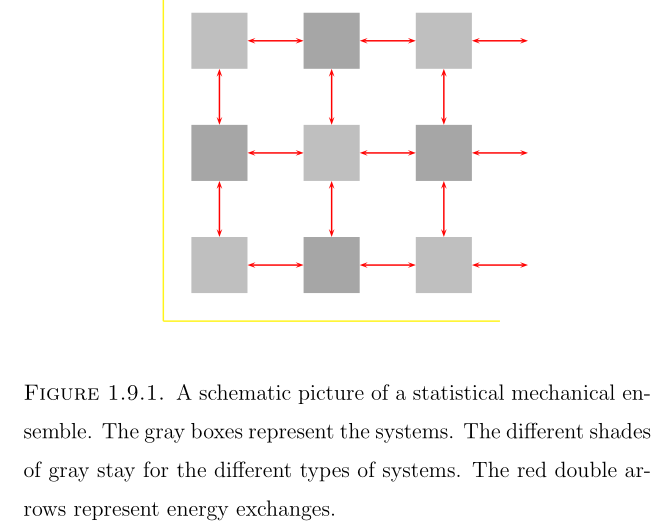
\includegraphics[width=0.5\textwidth]{pictures_1/fig 1.9.1.png}
    \label{fig:1.9.1}
\end{figure}


Statistical mechanics is based on an abstract model of ideal gas, construed as a system formed by a large number of almost non interacting molecules. The model however applies to any supersystem, called ensemble, that can be partitioned in a large number of weakly interacting parts, called systems. The ensemble are useful in a lot of situation, for example for the black body in witch the electromagnetic waves can be viewed as a "gas" of non-interacting harmonic oscillators.

An ensemble is a collection of a large number of systems, as shown in fig. 1.9.1. The systems can be of different types labelled by $\tau$. The systems of the same type are identical but distinguishable: they have the same physical properties but a distinct individuality, much as identical twins do. (for example in a system with two identical twins and two different job the conifuration twin A job C and twin B job D is different to twin B job C twin A job D) The number $N_{\tau}$ of systems of type $\tau$ is fixed: the systems can be neither created nor destroyed nor exchanged with the rest of the universe, this systems are called canonical systems, the gran canonical ones can exchange also matter (non sicuro sia gran canonico).

The states of the systems of type $\tau$ form a discrete set labelled by one or more indices denoted collectively by $s$ (Boltzmann believed that all in nature has quantized value). When a system of type $\tau$ is in the state $s$, it has an energy $e_{\tau s}$. The value of $e_{\tau s}$ depends on the external conditions $a_{x}$ on the systems, such as the volume available, applied force fields, etc.

Further, the ensemble is assumed to be in equilibrium. So, the amount of energy exchanged at any time by each system is small compared to the energy owned by the system. A mechanical state of the ensemble is specified by the states of the sum total of its constituent systems. A configuration $\underline{n}$ of the ensemble is a statistical property recording the numbers $n_{\tau s}$ of systems of each type $\tau$ in each state $s$. The configuration numbers $n_{\tau s}$ cannot be arbitrary. Indeed, since each system is always in one and only one state, one must have
 
\begin{equation*}
N_{\tau}=\sum_{s} n_{\tau s} \tag{1.9.1}
\end{equation*}
 

It is clear that each mechanical state of the ensemble determines a configuration $\underline{n}$, but not viceversa; a configuration is determined in general by very may states.

As the systems exchange only small amounts of energy, their interaction energy is negligible compared to their total energy. For this reason, the mechanical energy $U^{m}$ of the ensemble equals the total energy of the systems,

\begin{equation}
U^{m}=\sum_{\tau} \sum_{s} n_{\tau s} e_{\tau s} \tag{1.9.2}
\end{equation}

A configuration $\underline{n}$ of the ensemble is said compatible with the energy value $U^{m}$ if (1.9.2) holds. A state of the ensemble is compatible with $U^{m}$ if the associated configuration $\underline{n}$ is.

The basic problem of ensemble theory can be stated as follows: to determine the actual configuration of the ensemble when its energy is $U^{m}$. The solution is based on a theoretical hypothesis, validated a posteriori by the agreement of its prediction with evidence, the principle of equiprobability a priori of the mechanical states.


\footnotetext{
${ }^{2}$ In classical statistical mechanics, the set of states is continuous and is discretized here to make certain quantities well-defined. At the end, continuity will be restored. In quantum statistical mechanics, the set of state is instead truly discrete.
}

\textbf{At equilibrium, all the mechanical states of the ensemble compatible with an energy value $U^{m}$ have the same probability to occur}. Consequently,
\textbf{The probability of a configuration $\underline{n}$ of the ensemble compatible with $U^{m}$ to come about is proportional to the number $\Gamma(\underline{n})$ of mechanical states which determine that configuration.}

From here, it is possible to show that there is a most probable configuration $\underline{\underline{n}}$ of the ensemble and compute it. In fact, $\underline{\bar{n}}$ is the configuration that maximizes $\Gamma(\underline{n})$ or, what is the same, the Boltzmann entropy

\begin{equation}
S(\underline{n})=\ln \Gamma(\underline{n}) \tag{1.9.3}
\end{equation}

subject to the sum rules (1.9.1) and the energy condition (1.9.2). The solution of this constrained variational problem is

\begin{equation}
\bar{n}_{\tau s}=N_{\tau} \frac{\exp \left(-\beta e_{\tau s}\right)}{Z_{\tau}(\beta)} \tag{1.9.4}
\end{equation}

where $\bar{n}_{\tau s}$, and more in general the \bar{x} notation, indicate the most probable configuration. (temperature and entropy doesn't has a immediate correspondence with the mechanical approach but, using the Lagrange multiplier (because the maximization has constrains due to eq 1.9.1 and 1.9.2) we will see that $\beta$ (Lagrange coefficient) is related to the inverse of the temperature and $\Gamma(\underline{n})$ to entropy). $Z_{\tau}(\beta)$ is the canonical partition function of the type $\tau$ systems,

\begin{equation}
Z_{\tau}(\beta)=\sum_{s^{\prime}} \exp \left(-\beta e_{\tau s^{\prime}}\right) \tag{1.9.5}
\end{equation}

and $\beta$ is determined implicitly by imposing that the $\bar{n}_{\tau s}$, as given by eq. (1.9.4), satisfy (1.9.2). It is also possible to show that the most probable configuration $\underline{\bar{n}}$ of the ensemble is far more probable than any other one $\underline{n}$ compatible with $U^{m}$ so configuration $\underline{\bar{n}}$ is virtually the effective one.

From now on, we will stop specifying that $\underline{\bar{n}}$ is the most probable. Further, we conventionally denote any quantity $G^{m}$ depending on the configuration $\underline{n}$ of the ensemble by $\bar{G}^{m}$ when evaluated at the configuration $\underline{\bar{n}}$.

Is now necessary to introduce some hypotheses supported by physical reasoning and justified a posteriori by the increasing agreement of the predictions. The first hypotheses consist in the identification of the ensemble's mechanical energy $\bar{U}^{m}$ and thermodynamical internal energy $U$,

\begin{equation*}
\bar{U}^{m}=U \tag{1.9.25}
\end{equation*}

Assumed as selfevident because no other form of energy appear to be present, this because if $\bar{U}^{m}$ were different from $U$, the difference $\bar{U}^{m}-U$ would be a non mechanical form of energy explainable only through a more complicated and less predictive theory.

It is known from standard thermodynamics that the internal energy $U$ and
the external conditions $a_{x}$ constitute a set of thermodynamical coordinates: their assignment determines the thermodynamical state of the system. By (1.9.25), therefore, any thermodynamical state function can be expressed as a function of $\bar{U}^{m}$ and $a_{x}$ and any such function defines a thermodynamical state function.

The quantity $\beta$ is determined by (1.9.2) via (1.9.4) as a function of $\bar{U}^{m}$ and the $a_{x}$. Thus, $\beta$ is a thermodynamical state function.

The configuration $\underline{n}$ is determined by $\bar{U}^{m}$ and the $a_{x}$. Thus any quantity that is a function of $\underline{\bar{n}}$ is also a function of $\bar{U}^{m}$ and the $a_{x}$ and, so, a thermodynamical state function.

By the 1st law of thermodynamics, in an infinitesimal transformation of the ensemble's thermodynamical state, the variation $d U$ of the internal energy $U$ is

\begin{equation}
d U=\not d Q+\not d W \tag{1.9.26}
\end{equation}

where $\not d Q$, $\not d W$ are the heat and the work exchanged in the transformation, respectively. By (1.9.2), in the same transformation, the notation $\not d$ means not exact differential, the variation $d \bar{U}^{m}$ of the mechanical energy $\bar{U}^{m}$ is given by (making the deviates)

\begin{equation}
d \bar{U}^{m}=\sum_{\tau} \sum_{s} d \bar{n}_{\tau s} e_{\tau s}+\sum_{\tau} \sum_{s} \bar{n}_{\tau s} d e_{\tau s} \tag{1.9.27}
\end{equation}

where $d e_{\tau s}$ is the variation of $e_{\tau s}$ determined by the concurrent variation of the external conditions $a_{x}$. On account of (1.9.25), it should be possible to identify the contributions of the right hand sides of eqs. (1.9.26), (1.9.27). The comparison however is not straightforward. As is well-known from thermodynamics, $\not d Q$, $\not d W$ are not exact differentials, while $d \bar{n}_{\tau s}, d e_{\tau s}$ are. Thus, $\not d Q, \not d W$ depend on the nature of the transformation intervening between the given states, while $d \bar{n}_{\tau s}, d e_{\tau s}$ do not. So it is natural to assume that this transformation is a reversible one. Granting this, inspection of (1.9.26), (1.9.27) suggests the following theory.

In an infinitesimal reversible transformation, heat and work exchanges are the parts to $d \bar{U}^{m}$ due respectively to a variation $d \bar{n}_{\tau s}$ of the configuration numbers $\bar{n}_{\tau s}$ at fixed energies $e_{\tau s}$ and a variation de $e_{\tau s}$ of the energies $e_{\tau s}$ at fixed configuration numbers $\bar{n}_{\tau s}$,

\begin{equation}
 d Q_{\mathrm{rev}}=\sum_{\tau} \sum_{s} d \bar{n}_{\tau s} e_{\tau s}  \tag{1.9.28} 
 \end{equation}
 \begin{equation}
 d W_{\mathrm{rev}}=\sum_{\tau} \sum_{s} \bar{n}_{\tau s} d e_{\tau s} \tag{1.9.29} 
\end{equation}

the energy depends also by the external fields ($a_x$, is an hypothesis)

Relation (1.9.28) is the key to the identification of thermodynamical entropy.
Let us define the ensemble's statistical entropy by
 
\begin{equation*}
S^{m}=S(\underline{n}) \tag{1.9.30}
\end{equation*}
 

Then, $\bar{S}^{m}$ is a thermodynamical state function, but one of a non mechanical purely statistical nature. Now, $\bar{S}^{m}$ has the following remarkable property,
 
\begin{equation*}
\not d Q_{\mathrm{rev}}=\beta^{-1} d \bar{S}^{m} \tag{1.9.31}
\end{equation*}
 

Proof. By (1.9.30) and (1.9.7), we have (è corta e magari aiuta a capire quindi la lascio)
 
\begin{equation*}
d \bar{S}^{m}=-\sum_{\tau} \sum_{s} d \bar{n}_{\tau s} \ln \bar{n}_{\tau s} \tag{1.9.32}
\end{equation*}
 

Inserting (1.9.19) into (1.9.32), we obtain
 
\begin{equation*}
d \bar{S}^{m}=\sum_{\tau} \sum_{s} d \bar{n}_{\tau s}\left(\alpha_{\tau}+\beta e_{\tau s}\right)=\sum_{\tau} \alpha_{\tau} \sum_{s} d \bar{n}_{\tau s}+\beta \sum_{\tau} \sum_{s} d \bar{n}_{\tau s} e_{\tau s} \tag{1.9.33}
\end{equation*}
 

By (1.9.1), as the total number $N_{\tau}$ of units of each type $\tau$ remains constant, we have
 
\begin{equation*}
\sum_{s} d \bar{n}_{\tau s}=0 \tag{1.9.34}
\end{equation*}
 

Using (1.9.34) in (1.9.33) and recalling (1.9.28), we find
 
\begin{equation*}
d \bar{S}^{m}=\beta \sum_{\tau} \sum_{s} d \bar{n}_{\tau s} e_{\tau s}=\beta \not d Q_{\mathrm{rev}} \tag{1.9.35}
\end{equation*}
 
(1.9.31) follows.

Relation (1.9.31) is reminiscent of the well-known thermodynamical relation

\begin{equation}
\not d Q_{\mathrm{rev}}=T d S \tag{1.9.36}
\end{equation}

where $T$ and $S$ are the absolute temperature and the thermodynamical entropy of the ensemble. This suggests the identification of $\beta$ with $1 / T$ and $\bar{S}^{m}$ with $S$. This however cannot work for dimensional reasons. $\beta$ has the dimension of 1/energy while $T$ has the dimension of temperature; $\bar{S}^{m}$ is dimensionless while $S$ has the dimension of energy/temperature. Is so necessary to introduce a dimensional constant.

\begin{gather*}
\bar{S}^{m}=S / k_{B}  \tag{1.9.37}\\
\beta=1 / k_{B} T \tag{1.9.38}
\end{gather*}

where $k_{B}$ is a constant with the dimensions of energy/temperature, called Boltzmann constant.

\begin{equation*}
k_{B}=1.3806488(13) \times 10^{-16} \operatorname{erg}^{\circ} \mathrm{K}^{-1} \tag{1.9.39}
\end{equation*}

($1 erg= 10^-7J$)
The thermodynamical free energy (of helmholtz) of the ensemble is (used only for technical reason for simplify the results)

\begin{equation*}
F:=U-T S=\bar{U}^{m}-\beta^{-1} \bar{S}^{m} \tag{1.9.40}
\end{equation*}


Proof. Indeed, using (1.9.25), (1.9.37), (1.9.38), we have

\begin{equation*}
\bar{U}^{m}-\beta^{-1} \bar{S}^{m}=U-k_{B} T S / k_{B}=U-T S=F \tag{1.9.41}
\end{equation*}

as claimed.

The relevance of $F$ stems from its having a simple statistical expression,

\begin{equation*}
F=-\beta^{-1} \sum_{\tau} N_{\tau} \ln Z_{\tau}(\beta) \tag{1.9.42}
\end{equation*}


On account of (1.9.38), we write the free energy $F$ in (1.9.42) as

\begin{equation}
F=-k_{B} T \sum_{\tau} N_{\tau} \ln Z_{\tau} \tag{1.9.46}
\end{equation}

where the partition function $Z_{\tau}=Z_{\tau}\left(1 / k_{B} T\right)$ in (1.9.5) is now regarded as a thermodynamical state function,

\begin{equation*}
Z_{\tau}=\sum_{s^{\prime}} \exp \left(-\frac{e_{\tau s^{\prime}}}{k_{B} T}\right) \tag{1.9.47}
\end{equation*}


Once the free energy $F$ is known, one to compute the main thermodynamical state functions in statistical mechanics using well-known standard thermodynamical relations. For a gas of pressure $P$ in a volume $V$, these read
 
\begin{align*}
U & =F-T\left(\frac{\partial F}{\partial T}\right)_{V}=-T^{2}\left(\frac{\partial}{\partial T} \frac{F}{T}\right)_{V}  \tag{1.9.48}\\
S & =-\left(\frac{\partial F}{\partial T}\right)_{V}  \tag{1.9.49}\\
P & =-\left(\frac{\partial F}{\partial V}\right)_{T} \tag{1.9.50}
\end{align*}
 

\subsection*{1.10. Elementary applications of statistical mechanics}

In this section, we shall illustrate a few simple applications of the theoretical framework of statistical mechanics expounded in sect. 1.9

Consider a chemically pure (so the $\tau$ index doesn't appear, identical molecules) ideal (he molecules are weakly interacting) gas of pointlike molecules. The dynamical state of a molecule is specified by its position $\boldsymbol{q}$ and momentum $\boldsymbol{p}$, that is by its phase. The energy of a molecule in such a state reduces to its kinetic energy,

\begin{equation*}
e(\boldsymbol{p})=\frac{\boldsymbol{p}^{2}}{2 m} \tag{1.10.1}
\end{equation*}

where $m$ is the molecular mass.

The application of the formal methods of statistical mechanics to the study of the gas begins with the calculation of its partition function $Z$. By (1.9.47), on account of (1.10.1), this is given by (passing from discrete to continue quantities because of the huge number of molecules)

\begin{equation*}
Z=\int d^{3} \boldsymbol{q} \int d^{3} \boldsymbol{p} \exp \left(-\frac{\boldsymbol{p}^{2}}{2 m k_{B} T}\right) \tag{1.10.2}
\end{equation*}

$Z$ can be computed easily,

\begin{equation*}
Z=V\left(2 \pi m k_{B} T\right)^{3 / 2} \tag{1.10.3}
\end{equation*}


Proof. The $\boldsymbol{q}$ integration is trivial, since the integrand is $\boldsymbol{q}$ independent, and gives a factor $V$. The $\boldsymbol{p}$ integration is Gaussian and can be carried out using the formula
 
\begin{equation*}
\int d^{n} x \exp \left(-\frac{a}{2} x^{2}\right)=(2 \pi / a)^{n / 2} \tag{1.10.4}
\end{equation*}
 
producing a further factor $\left(2 \pi m k_{B} T\right)^{3 / 2}$.

By (1.9.4), taking (1.10.1), (1.10.3) into account, the fraction of molecules whose coordinates and momenta lie in the small volumes $d^{3} \boldsymbol{q}, d^{3} \boldsymbol{p}$ around $\boldsymbol{q}, \boldsymbol{p}$ is
 
\begin{equation*}
f_{\mathrm{ps}}(\boldsymbol{q}, \boldsymbol{p}) d^{3} \boldsymbol{q} d^{3} \boldsymbol{p}=\frac{1}{V\left(2 \pi m k_{B} T\right)^{3 / 2}} \exp \left(-\frac{\boldsymbol{p}^{2}}{2 m k_{B} T}\right) d^{3} \boldsymbol{q} d^{3} \boldsymbol{p} \tag{1.10.5}
\end{equation*}
 

From here, integrating with respect to $\boldsymbol{q}$, it follows that the fraction of molecules whose momenta lie in the the volume $d^{3} \boldsymbol{p}$ around $\boldsymbol{p}$ is
 
\begin{equation*}
f_{\mathrm{ms}}(\boldsymbol{p}) d^{3} \boldsymbol{p}=\frac{1}{\left(2 \pi m k_{B} T\right)^{3 / 2}} \exp \left(-\frac{\boldsymbol{p}^{2}}{2 m k_{B} T}\right) d^{3} \boldsymbol{p} \tag{1.10.6}
\end{equation*}
 

This is the molecular momentum Maxwell distribution (J. C. Maxwell, 1860). The fraction of molecules whose energy lies in the small interval de around $e$ is
 
\begin{equation*}
f_{\mathrm{e}}(e) d e=\frac{2}{\pi^{1 / 2}\left(k_{B} T\right)^{3 / 2}} \exp \left(-\frac{e}{k_{B} T}\right) e^{1 / 2} d e \tag{1.10.7}
\end{equation*}
 

This is the molecular energy Maxwell distribution, which is plotted in fig. 1.10.1.

Proof. In spherical coordinates, the momentum space elementary volume $d^{3} \boldsymbol{p}$ is $d p p^{2} d \vartheta \sin \vartheta d \varphi$. Here, $d p p^{2}=d p^{2} p / 2=(2 m)^{3 / 2} d e e^{1 / 2} / 2$. Further, angular integration gives a factor $4 \pi$. Then, (1.10.7) follows immediately from (1.10.6).

\begin{figure}[h!]
    \centering
    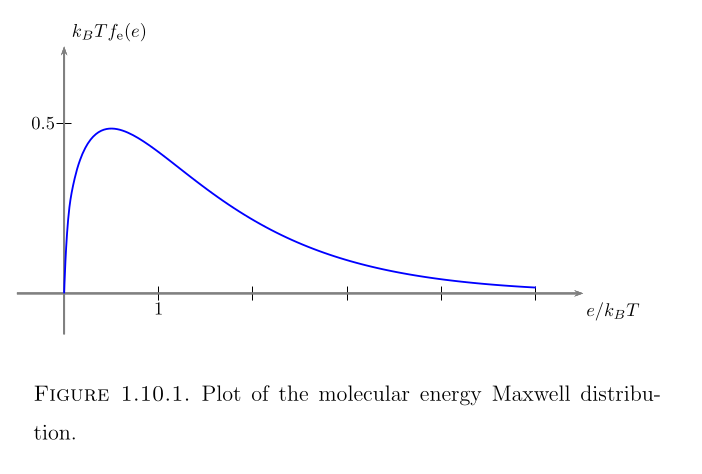
\includegraphics[width=0.5\textwidth]{pictures_1/fig 1.10.1.png}
    \label{fig:1.9.1}
\end{figure}

Substituting (1.10.3) in (1.9.46), we obtain the free energy of the gas,
 
\begin{equation*}
F=-N k_{B} T\left[\ln V+\frac{3}{2} \ln T+\frac{3}{2} \ln \left(2 \pi m k_{B}\right)\right] \tag{1.10.8}
\end{equation*}
 
where $N$ is the number of molecules of the gas. Using the thermodynamical relations (1.9.48)-(1.9.50), we obtain readily the expressions of the internal energy, entropy and pressure of the gas,
 
\begin{align*}
U & =\frac{3}{2} N k_{B} T  \tag{1.10.9}\\
S & =N k_{B}\left[\ln V+\frac{3}{2} \ln T+\frac{3}{2} \ln \left(2 \pi m k_{B}\right)+\frac{3}{2}\right]  \tag{1.10.10}\\
P & =\frac{N k_{B} T}{V} \tag{1.10.11}
\end{align*}
 
${ }^{3}$. A couple of important remarks are in order.
Eq. (1.10.9) is in agreement with the so called equipartition theorem, which states that the kinetic energy per degree of freedom is $k_{B} T / 2$. The gas has $3 N$ degrees of freedom and, being ideal, its energy reduces to the kinetic one. Thus, by the theorem, its energy is necessarily $3 N k_{B} T / 2$.

Eq. (1.10.11) can be recognized as the ideal gas state equation (in thermodynamics this is a phenomenological relation but proceeding in this way we have reached the same result as a theorem, this kind of thing validated our hypothesis's a posteriori)
 
\begin{equation*}
P=\frac{n R T}{V} \tag{1.10.12}
\end{equation*}
 
where $n$ is the number of moles forming the gas and $R$ is the universal gas constant
 
\begin{equation*}
R=8.3144621(75) \times 10^{7} \mathrm{erg}^{\circ} \mathrm{K}^{-1} \mathrm{~mol}^{-1} \tag{1.10.13}
\end{equation*}
 

\footnotetext{
${ }^{3}$ The expression (1.10.10) of $S$ is actually wrong, because $S$, as given by $(1.10 .10)$, is not extensive. This failure of classical statistical mechanics is due to considering the molecules as identical but distinguishable. In quantum statistical mechanics, where the molecules are assumed instead to be identical and indistinguishable, the correct extensive form is obtained. The term $\ln V$ gets replaced by $\ln (V / N)$ and the entropy's extensiveness is recovered.
}

The mole number $n$ of the gas is given by
 
\begin{equation*}
n=N / N_{A} \tag{1.10.14}
\end{equation*}
 
where $N_{A}$ is the number of molecules of a mole, which has a universal value, as discovered by A. Avogadro's in 1811. The Avogadro's number can be computed by a variety of means,
 
\begin{equation*}
N_{A}=6.02214129(27) \times 10^{23} \mathrm{~mol}^{-1} \tag{1.10.15}
\end{equation*}
 

It follows that
 
\begin{equation*}
k_{B}=R / N_{A} \tag{1.10.16}
\end{equation*}
 
from which the value (1.9.39) can be obtained.

The second (important) example is based on an ideal gas of 1-dimensional harmonic oscillators of a single specie . Since they are identical, the oscillators are of a single type. Since the gas is ideal, the oscillators are weakly interacting. The dynamical state of an oscillator is specified by its position $q$ and momentum $p$, that is by its phase. The energy of an oscillator in such a state is given by the well-known relation
 
\begin{equation*}
e(q, p)=\frac{p^{2}}{2 m}+\frac{1}{2} m \omega^{2} q^{2} \tag{1.10.17}
\end{equation*}
 
where $m$ and $\omega$ are the oscillator's mass and angular frequency. The gas is so an ensemble constituted by systems of a unique type. There is thus no need to keep track of type in calculations.

By (1.9.47), using (1.10.17), the partition function of the gas is
 
\begin{equation*}
Z=\int d q \int d p \exp \left[-\frac{1}{k_{B} T}\left(\frac{p^{2}}{2 m}+\frac{1}{2} m \omega^{2} q^{2}\right)\right] \tag{1.10.18}
\end{equation*}
 
$Z$ can be computed easily,
 
\begin{equation*}
Z=\frac{2 \pi k_{B} T}{\omega} \tag{1.10.19}
\end{equation*}
 
Both the $q$ and the $p$ integrals are Gaussian and can be computed using the formula (1.10.4).

By (1.9.4), taking (1.10.17), (1.10.19) into account, the fraction of oscillators whose coordinates and momenta lie in the small intervals $d q, d p$ around $q, p$ is
 
\begin{equation*}
f_{\mathrm{ps}}(q, p) d q d p=\frac{\omega}{2 \pi k_{B} T} \exp \left[-\frac{1}{k_{B} T}\left(\frac{p^{2}}{2 m}+\frac{1}{2} m \omega^{2} q^{2}\right)\right] d q d p \tag{1.10.20}
\end{equation*}
 

From here, one can easily compute the fraction of oscillators whose energy $e$ and phase angle $\varphi$ lie in the small intervals $d e, d \varphi$ around $e, \varphi$
 
\begin{equation*}
f_{\mathrm{ea}}(e, \varphi) \operatorname{ded} \varphi=\frac{1}{2 \pi k_{B} T} \exp \left(-\frac{e}{k_{B} T}\right) d e d \varphi \tag{1.10.21}
\end{equation*}
 

Proof. The energy $e$ and phase angle $\varphi$ of an oscillator are (lascio la dim perchè credo che qualche esercizio potrebbe basarsi su questi calcoli)
 
\begin{equation*}
e=\frac{p^{2}}{2 m}+\frac{1}{2} m \omega^{2} q^{2}, \quad \varphi=\tan ^{-1}\left(\frac{p}{m \omega q}\right) \tag{1.10.22}
\end{equation*}
 

The standard coordinate and momentum $q, p$ can be expressed in terms of these as
 
\begin{equation*}
q=\left(\frac{2 e}{m \omega^{2}}\right)^{1 / 2} \cos \varphi, \quad p=(2 m e)^{1 / 2} \sin \varphi \tag{1.10.23}
\end{equation*}
 
Because we can consider the phase space (spazio delle fasi non so il termine tecnico).
From here, we deduce immediately that
 
\begin{align*}
d q d p & =\left|\frac{\partial q}{\partial e} \frac{\partial p}{\partial \varphi}-\frac{\partial q}{\partial \varphi} \frac{\partial p}{\partial e}\right| d e d \varphi  \tag{1.10.24}\\
& =\left|\left(\frac{1}{2 m e \omega^{2}}\right)^{1 / 2} \cos \varphi(2 m e)^{1 / 2} \cos \varphi+\left(\frac{2 e}{m \omega^{2}}\right)^{1 / 2} \sin \varphi\left(\frac{m}{2 e}\right)^{1 / 2} \sin \varphi\right| \operatorname{ded} \varphi \\
& =\frac{1}{\omega} d e d \varphi
\end{align*}
 

Substituting (1.10.23), (1.10.24) in (1.10.20), we reach (1.10.21).

Integrating $f_{\text {ea }}(e, \varphi)$ with respect to $\varphi$, we obtain the oscillator energy distribution
 
\begin{equation*}
f_{\mathrm{e}}(e) d e=\frac{1}{k_{B} T} \exp \left(-\frac{e}{k_{B} T}\right) d e \tag{1.10.25}
\end{equation*}
 

\begin{figure}[h!]
    \centering
    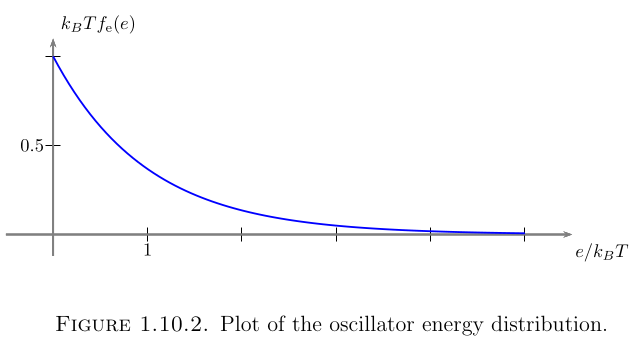
\includegraphics[width=0.5\textwidth]{pictures_1/fig 1.10.2.png}
    \label{fig:1.9.1}
\end{figure}

Figure 1.10.2. Plot of the oscillator energy distribution.
This is plotted in fig. 1.10.2.
Substituting (1.10.19) in (1.9.46), we obtain the free energy of the gas,
 
\begin{equation*}
F=-N k_{B} T\left[\ln T+\ln \left(\frac{2 \pi k_{B}}{\omega}\right)\right] \tag{1.10.26}
\end{equation*}
 
where $N$ is the number of oscillators of the gas. Using the thermodynamical relations (1.9.48), (1.9.49), we obtain readily the expressions of the internal energy, entropy and pressure of the gas,
 
\begin{align*}
U & =N k_{B} T  \tag{1.10.27}\\
S & =N k_{B}\left[\ln T+\ln \left(\frac{2 \pi k_{B}}{\omega}\right)+1\right] \tag{1.10.28}
\end{align*}
 

Note that a pressure is not defined for a gas of oscillators, since a volume cannot be assigned to it and the free energy does not depend on the volume $V$. The expression $(1.10 .27)$ can also be interpreted in the light of the equipartition theorem. 


\subsection*{1.11. The black body radiation and the beginning of quantum physics}

In a warm body, the collisions of the molecules cause the acceleration of their charged constituents which consequently emit electromagnetic waves. The resulting energy loss suffered by the molecules decreases their energy and so attenuates their thermal agitation. In turn, electromagnetic waves are absorbed by the molecular charges which consequently get accelerated. The ensuing energy gain undergone by the molecules increases their energy and contributes to their thermal motion. Thermal radiation is the electromagnetic radiation field surrounding one or more warm bodies that results from these concomitant processes. Because of its relation to thermal motion, thermal radiation is essentially a thermal phenomenon.

Electromagnetic waves are endowed with energy and the waves' propagation involves an energy flux. If several bodies of different temperatures are put at close distance from each other, they exchange energy because of the energy flux inherent in the thermal radiation they generate. The warmer ones get cooler by releasing more energy than they acquire, the cooler ones get warmer by acquiring more energy than they release. This is a form heat transfer and continues until all bodies acquire the same temperature. The bodies are then in mutual thermodynamical equilibrium.

In the neighborhood of a collection of warm bodies in equilibrium, the thermal radiation is approximately isotropic, that is it has the same properties in all directions. Note that equilibrium is necessary for isotropy.

Since thermal radiation is a form of electromagnetic radiation, it is to electromagnetic waves which we have to turn to for a better understanding of it.

An electromagnetic wave is a superposition of monochromatic electromagnetic waves of all possible frequencies. The dynamics of the monochromatic components of the wave is governed by the wave equation (1.2.1) as when they are
isolated from each other rather than superposed together (cf. sect 1.2). The components are thus non interacting, since an interaction would inevitably alter their dynamics. They so contribute separately and independently to all the wave's additive quantities, in particular to the wave's energy and momentum and energy and momentum flow. The contribution to such quantities of the components with frequency lying in a short range $\omega$ to $\omega+\Delta \omega$ is then unambiguously determined and the quantities can thus be expressed as integrals of monochromatic contributions over the whole frequency spectrum.

A warm body in equilibrium does not release energy as isotropic thermal radiation uniformly at all frequencies. The energy belonging to the small frequency range from $\omega$ to $\omega+\Delta \omega$ emitted by the unit area of the body's surface in the unit time is proportional to $\Delta \omega$ and so expressible as $z_{\omega} \Delta \omega . z_{\omega}$ is called isotropic spectral emissive power. Besides $\omega, z_{\omega}$ is a function of the body's temperature $T$. As such, it is non universal, depending on the body's physical features.

The energy flow of the isotropic thermal radiation getting to a worm body in equilibrium is not equally intense at all frequencies either. The amount of energy of the radiation in the small frequency range from $\omega$ to $\omega+\Delta \omega$ reaching the unit area of the body's surface in the unit time is proportional to $\Delta \omega$ and so representable as $H_{\omega} \Delta \omega$. $H_{\omega}$ is called isotropic spectral energy flux density.

When thermal radiation reaches a warm body, a part of it is absorbed, a part is transmitted and a part is reflected. The body does not absorb energy from the isotropic thermal radiation uniformly at all frequencies. The fraction $\alpha_{\omega}$ of the energy $H_{\omega} \Delta \omega$ that is absorbed is is called absorptive power and is also a non universal function of $T$.

A black body is an ideal body with maximum absorptive power,
 
\begin{equation*}
\alpha_{B \omega}=1 \tag{1.11.1}
\end{equation*}
 

In other words, a black body is a perfect absorber. As we shall see soon, a black body is also a perfect emitter. Further, as any body, a black body emits thermal
radiation known as black body radiation.
Suppose that a body $a$, not necessarily black, is placed in the vicinity of a black body $b$. Suppose further that $a$ and $b$ have the same temperature and are hence in equilibrium. Then,
 
\begin{equation*}
z_{a \omega}=\alpha_{a \omega} z_{b \omega} \tag{1.11.2}
\end{equation*}
 

This relation is known as Kirchhoff theorem (G. Kirchhoff, 1859).

Proof. At equilibrium, by energy conservation, the energy in the frequency range from $\omega$ to $\omega+\Delta \omega$ emitted per unit surface area and time by the body $a, z_{a \omega} \Delta \omega$, equals the energy in the same frequency range absorbed per unit surface area and time by $a$, $\alpha_{a \omega} H_{\omega} \Delta \omega$. Hence, we have $z_{a \omega}=\alpha_{a \omega} H_{\omega}$. Reasoning in the same for the black body $b$, we find that similarly $z_{b \omega}=\alpha_{b \omega} H_{\omega}$. Since $b$ is black, however, $\alpha_{b \omega}=1$ by (1.11.1). It follows so that $z_{b \omega}=H_{\omega}$. Combining the expressions for $z_{a \omega}, z_{b \omega}$ we obtained aboev, we conclude that $z_{a \omega}=\alpha_{a \omega} z_{b \omega}$ proving relation (1.11.2).

Kirchhoff theorem has two important consequences.
Black bodies have all the same emissive power $z_{B \omega}$, which is consequently a universal function of their temperature $T$.

Proof. If $a$ is a black body too, then $\alpha_{a \omega}=1$ by (1.11.1) and, so, $z_{a \omega}=z_{b \omega}$, by (1.11.2). The statement is thus obvious.

A black body is a perfect emitter.

Proof. If $a$ is generic body, $\alpha_{a \omega} \leq 1$ and consequently $z_{a \omega} \leq z_{B \omega}$ on account of (1.11.2). It follows that the universal black body emissive power is the highest possible.

![](https://cdn.mathpix.com/cropped/2024_09_22_5d1e855547710648961eg-0071.jpg?height=440&width=578&top_left_y=531&top_left_x=817)

Figure 1.11.1. A large cavity $C$ with a small aperture $A$ behaves as a black body, since all radiation entering $C$ through $A$ cannot leave $C$ and is thus effectively absorbed. The radiation in $C$ probed through $A$ is thus black body radiation.

At room temperature, a black body appears black, as most of the frequencies which it radiates are infrared and cannot be perceived by the human eye. At higher temperatures, however, a black body glows increasingly exhibiting colors that range from dark red to bright blue-white as temperature increases. The sun behaves as a black body.

An approximate realization of a black body is a large cavity with a small hole pierced in one of its walls, as shown schematically in fig. 1.11.1. The thermal radiation entering the cavity through the hole is either reflected indefinitely or absorbed by the cavity's walls and, so, it is unlikely to reemerge. The aperture of the cavity behaves therefore an almost perfect absorber and, so, comes close to be a black body. The thermal radiation coming out from the cavity through the aperture is therefore nearly black body radiation. Note that total absorption of the incoming radiation is compatible with the concomitant emission of it.

From now on, we shall consider black bodies only and suppress the suffix $B$ marking black body quantities throughout.

The main problem of black body theory is the determination of the emissive
power $z_{\omega}$ as a function of temperature $T$. As it turns out, its solution proceeds through the study of black body radiation and in particular of the latter's energy density, as we show next

The contribution of the components of the small frequency range from $\omega$ to $\omega+\Delta \omega$ to the radiation's energy density is proportional to $\Delta \omega$ and so expressible as $u_{\omega} \Delta \omega . u_{\omega}$ is called isotropic spectral energy density. Significantly, the black body emissive power $z_{\omega}$ stands in a simple relation to $u_{\omega}$,
 
\begin{equation*}
z_{\omega}=\frac{c u_{\omega}}{4} \tag{1.11.3}
\end{equation*}
 

Proof. Since the black body radiation is isotropic, the spectral energy density $u_{\omega}$ is built up uniformly by the radiation flowing in all possible directions. The contribution to $u_{\omega}$ of the radiation flowing within a certain solid angle $\Delta o$ is thus $u_{\omega} \Delta o / 4 \pi$, since $\Delta o / 4 \pi$ is the fractional weight of $\Delta o$. As shown in fig. 1.11.2, the electromagnetic energy emitted in the frequency range from $\omega$ to $\omega+\Delta \omega$ by the area $\Delta A$ of the black body's surface in the time $\Delta t$ within the solid angle $\Delta o$ directed along the unit vector $\boldsymbol{e}_{r}, \Delta z_{\omega} \Delta \omega \Delta A \Delta t$, equals the electromagnetic energy relative to the same frequencies contained in the volume $\Delta V$ of the cylinder of base area $\Delta A$ and length $c \Delta t$ slanted along the direction $\boldsymbol{e}_{r}, u_{\omega} \Delta \omega \Delta V$, times the weight $\Delta o / 4 \pi$ of $\Delta o$,
 
\begin{equation*}
\Delta z_{\omega} \Delta \omega \Delta A \Delta t=u_{\omega} \Delta \omega \Delta V \frac{\Delta o}{4 \pi} \tag{1.11.4}
\end{equation*}
 
$\Delta z_{\omega}$ is the contribution to $z_{\omega}$ provided by the radiation emitted within the solid angle $\delta o$. Multiplication of the energy $u_{\omega} \Delta \omega \Delta V$ contained in the cylinder by the weight $\Delta o / 4 \pi$ is mandated by the fact this energy is not entirely yielded by the radiation emitted by the black body' surface through $\Delta o$. Only the fraction $\Delta o / 4 \pi$ of it is. Inspecting fig. 1.11.2, we find that
 
\begin{equation*}
\Delta V=\Delta A e_{3} \cdot c \Delta t e_{r} \tag{1.11.5}
\end{equation*}
 

Substituting (1.11.5) into (1.11.4), we find
 
\begin{equation*}
\Delta z_{\omega}=\frac{c u_{\omega}}{4 \pi} \boldsymbol{e}_{3} \cdot \boldsymbol{e}_{r} \Delta o \tag{1.11.6}
\end{equation*}
 

![](https://cdn.mathpix.com/cropped/2024_09_22_5d1e855547710648961eg-0073.jpg?height=611&width=942&top_left_y=513&top_left_x=575)

Figure 1.11.2. The elemental volume $\Delta V$.
To compute the total emissive power $z_{\omega}$, we integrate the contributions $\Delta z_{\omega}$ over all elemental solid angles $\Delta o$ in the half space above the body's surface. The geometry is shown in fig. 1.11.3. Using that $\Delta o=d \varphi d \vartheta \sin \vartheta, \boldsymbol{e}_{3} \cdot \boldsymbol{e}_{r}=\cos \vartheta$ with $\varphi$ and $\vartheta$ varying in the ranges $[0,2 \pi]$ and $[0, \pi / 2]$, we obtain
 
\begin{equation*}
z_{\omega}=\frac{c u_{\omega}}{4 \pi} \int_{0}^{2 \pi} d \varphi \int_{0}^{\pi / 2} d \vartheta \sin \vartheta \cos \vartheta=\frac{c u_{\omega}}{4} \tag{1.11.7}
\end{equation*}
 
proving (1.11.3).

The black body radiation can be considered on a par to a gas. We can confine the radiation in a cavity with perfectly reflecting walls, which works as its container. If the cavity has a volume $V$, the radiation has the volume $V$. If the radiation has been emitted by a black body at temperature $T$ at equilibrium, then the radiation can be attributed the temperature $T$. The energy of the electromagnetic field of the radiation can be identified with the radiation's internal energy $U$. The reflection of the radiation by the cavity's walls causes a momentum transfer from the field to these latter resulting in the radiation's pressure $P$. It makes thus sense to treat the black body radiation as an ordinary gas applying

![](https://cdn.mathpix.com/cropped/2024_09_22_5d1e855547710648961eg-0074.jpg?height=692&width=817&top_left_y=486&top_left_x=643)

Figure 1.11.3. The elemental solid angle $\Delta o$ in spherical coordinates.
the methods of thermodynamics and eventually of statistical mechanics.
Radiation pressure is a most relevant quantity in the thermodynamics of the black body radiation. Since pressure arises from momentum transfer from the radiation to the cavity's walls during reflection, the monochromatic components of the radiation contribute separately and independently to it by virtue of momentum additivity. The contribution of the components in the small frequency range from $\omega$ to $\omega+\Delta \omega$ to the radiation pressure is thus unambiguously determined and reads as $P_{\omega} \Delta \omega . P_{\omega}$ is called isotropic spectral radiation pressure.

Similarly, the contribution of the components of the small frequency range from $\omega$ to $\omega+\Delta \omega$ to the radiation's momentum density is proportional to $\Delta \omega$ and so representable as $g_{\omega} \Delta \omega . g_{\omega}$ is called isotropic spectral momentum density. The emergence of radiation pressure from momentum transfer from the radiation to the container's walls suggests that the spectral radiation pressure $P_{\omega}$ should be simply related to $g_{\omega}$. Indeed, one has
 
\begin{equation*}
P_{\omega}=\frac{c g_{\omega}}{3} \tag{1.11.8}
\end{equation*}
 

Proof. As the spectral energy density $u_{\omega}$, the spectral momentum density $g_{\omega}$ is built up uniformly by the radiation flowing in all possible directions. The contribution to $g_{\omega}$ of the radiation flowing within a certain solid angle $\Delta o$ is thus $g_{\omega} \Delta o / 4 \pi$. Examing fig. 1.11.2, it appears that the electromagnetic momentum pertaining the frequency range from $\omega$ to $\omega+\Delta \omega$ reaching the area $\Delta A$ of the walls in the time $\Delta t$ from within the solid angle $\Delta o$ directed along the unit vector $\boldsymbol{e}_{r}, \Delta \boldsymbol{G}$, equals the momentum associated to the same frequencies contained in the volume $\Delta V$ of the cylinder of base area $\Delta A$ and length $c \Delta t$ slanted in the direction $\boldsymbol{e}_{r}, g_{\omega} \Delta \omega \Delta V$, times the fractional weight of the solid angle $\Delta o, \Delta o / 4 \pi$, times $-\boldsymbol{e}_{r}$. So,
 
\begin{equation*}
\Delta \boldsymbol{G}=-g_{\omega} \Delta \omega \Delta V \frac{\Delta o}{4 \pi} \boldsymbol{e}_{r} \tag{1.11.9}
\end{equation*}
 

Multiplication of the momentum $u_{\omega} \Delta \omega \Delta V$ contained in the cylinder by the weight $\Delta o / 4 \pi$ is imposed by the consideration that not all momentum contained in the cylinder contributes to the momentum flowing to the wall from within $\Delta o$. Only the fraction $\Delta o / 4 \pi$ of it does. $\Delta V$ is given again by eq. (1.11.5), which we report here
 
\begin{equation*}
\Delta V=\Delta A \boldsymbol{e}_{3} \cdot c \Delta t \boldsymbol{e}_{r} \tag{1.11.10}
\end{equation*}
 

Substituting (1.11.10) into (1.11.9), we find
 
\begin{equation*}
\Delta \boldsymbol{G}=-\frac{c g_{\omega}}{4 \pi} \Delta \omega \Delta A \Delta t \Delta o \boldsymbol{e}_{3} \cdot \boldsymbol{e}_{r} \boldsymbol{e}_{r} \tag{1.11.11}
\end{equation*}
 

In a cavity with perfectly reflecting walls, the reflection of the black body radiation on a wall involves the inversion of the component of radiation's momentum normal to the wall, hence the momentum transfer to the wall manifesting as pressure. The radiation spectral pressure from the directions within the solid angle $\Delta o$ is thus
 
\begin{equation*}
\Delta P_{\omega}=\frac{\Delta G_{\mathrm{tr}}}{\Delta \omega \Delta A \Delta t} \tag{1.11.12}
\end{equation*}
 
where $\Delta G_{\mathrm{tr}}$ is the momentum transferred to $\Delta A$ during $\Delta t$ by the radiation coming from those directions, which is given by
 
\begin{equation*}
\Delta G_{\mathrm{tr}}=-2 e_{3} \cdot \Delta \boldsymbol{G} \tag{1.11.13}
\end{equation*}
 

The minus sign being introduced to render $\Delta G_{\mathrm{tr}}$ a non negative quantity. Substituting
(1.11.11) into (1.11.12), we find that
 
\begin{equation*}
\Delta P_{\omega}=\frac{c g_{\omega}}{2 \pi}\left(e_{3} \cdot e_{r}\right)^{2} \Delta o \tag{1.11.14}
\end{equation*}
 

To compute the total spectral pressure $P_{\omega}$, we integrate the contributions $\Delta P_{\omega}$ over all elemental solid angles $\Delta o$ in the half space on the internal side of the wall. The geometry is shown again in fig. 1.11.3. Using that $\Delta o=d \varphi d \vartheta \sin \vartheta, \boldsymbol{e}_{3} \cdot \boldsymbol{e}_{r}=\cos \vartheta$ with $\varphi$ and $\vartheta$ varying in the ranges $[0,2 \pi]$ and $[0, \pi / 2]$, we obtain
 
\begin{equation*}
P_{\omega}=\frac{c g_{\omega}}{2 \pi} \int_{0}^{2 \pi} d \varphi \int_{0}^{\pi / 2} d \vartheta \sin \vartheta \cos ^{2} \vartheta=\frac{c g_{\omega}}{3} \tag{1.11.15}
\end{equation*}
 
showing $(1.11 .8)$.

Because of the familiar energy to momentum relationship, for the isotropic electromagnetic relation which we are studying the spectral momentum density $g_{\omega}$ is related to the spectral energy density $u_{\omega}$ simply as
 
\begin{equation*}
u_{\omega}=c g_{\omega} \tag{1.11.16}
\end{equation*}
 

Proof. In mechanics, the kinetic energy $e$ of a system is a function of its momentum $\boldsymbol{p}$ and $\boldsymbol{v}=\boldsymbol{\nabla}_{\boldsymbol{p}} e$ is its velocity. As the electromagnetic radiation field can be considered as a free mechanical system, its spectral energy density $u_{\omega}$ must be a function of its spectral momentum density $g_{\omega}$. The derivative $d u_{\omega} / d g_{\omega}$ is in this case the light speed,
 
\begin{equation*}
\frac{d u_{\omega}}{d g_{\omega}}=c \tag{1.11.17}
\end{equation*}
 

This differential equation can be immediately integrated and the relation $u_{\omega}=c g_{\omega}+u_{\omega 0}$ is obtained, where $u_{\omega 0}$ is an integration constant. The spectral densities $u_{\omega}$ and $g_{\omega}$ are functions of the magnitude of the electric and magnetic field which vanish when both of these vanish. Thus, if $g_{\omega}$ vanishes, also $u_{\omega}$ does. Thus, $u_{\omega 0}=0$. Eq. (1.11.16) follows.

Combining (1.11.8), (1.11.16), we obtain
 
\begin{equation*}
P_{\omega}=\frac{u_{\omega}}{3} \tag{1.11.18}
\end{equation*}
 

The total energy density $u$ of the black body radiation is obtained by integration on the whole frequency spectrum of the spectral energy density $u_{\omega}$,
 
\begin{equation*}
u=\int_{0}^{\infty} d \omega u_{\omega} \tag{1.11.19}
\end{equation*}
 

Similarly, the total pressure $P$ of the radiation is given by
 
\begin{equation*}
P=\int_{0}^{\infty} d \omega P_{\omega} \tag{1.11.20}
\end{equation*}
 
(1.11.18) thus implies that
 
\begin{equation*}
P=\frac{u}{3} \tag{1.11.21}
\end{equation*}
 
which is the black body radiation's state equation.
The Stefan-Boltzmann law (J. Stefan, 1879) states that the total emissive power of a black body grows as the 4 -th power of temperature,
 
\begin{equation*}
z=\int_{0}^{\infty} d \omega z_{\omega}=\sigma T^{4} \tag{1.11.22}
\end{equation*}
 
where $\sigma$ is Stefan-Boltzmann constant, whose experimental value is
 
\begin{equation*}
\sigma=5.670373(21) \times 10^{-5} \mathrm{erg} \mathrm{cm}^{-2} \mathrm{sec}^{-1}{ }^{\circ} \mathrm{K}^{-4} \tag{1.11.23}
\end{equation*}
 

By (1.11.3) and (1.11.19), the black body radiation energy density is so
 
\begin{equation*}
u=\frac{4 \sigma}{c} T^{4} \tag{1.11.24}
\end{equation*}
 

The relation can be obtained theoretically (L. Boltzmann, 1884).

Proof. As we have remarked, the black body radiation is a thermodynamical system. In an infinitesimal transformation, the relation
 
\begin{equation*}
T d S=d U+P d V \tag{1.11.25}
\end{equation*}
 
holds. Substituting the relation (1.11.21) in (1.11.25) and recalling that $u$ is a function of temperature only and $U=u V$, we find
 
\begin{equation*}
T d S=V d u+u d V+\frac{1}{3} u d V=V \frac{d u}{d T} d T+\frac{4}{3} u d V \tag{1.11.26}
\end{equation*}
 

From (1.11.26), we read off the relations
 
\begin{equation*}
\left(\frac{\partial S}{\partial T}\right)_{V}=\frac{V}{T} \frac{d u}{d T}, \quad\left(\frac{\partial S}{\partial V}\right)_{T}=\frac{4 u}{3 T} \tag{1.11.27}
\end{equation*}
 
which in turn imply that
 
\begin{equation*}
\left(\frac{\partial}{\partial V}\right)_{T}\left(\frac{V}{T} \frac{d u}{d T}\right)=\left(\frac{\partial}{\partial V}\right)_{T}\left(\frac{\partial S}{\partial T}\right)_{V}=\left(\frac{\partial}{\partial T}\right)_{V}\left(\frac{\partial S}{\partial V}\right)_{T}=\left(\frac{\partial}{\partial T}\right)_{V}\left(\frac{4 u}{3 T}\right) \tag{1.11.28}
\end{equation*}
 

Computing the derivatives in (1.11.28), we find that $u$ satisfies the differential equation
 
\begin{equation*}
\frac{d u}{d T}=\frac{4 u}{T} \tag{1.11.29}
\end{equation*}
 
whose solution leads to (1.11.24) with $\sigma$ an integration constant.

The universality of the black body emissive power $z_{\omega}$ entails that of the radiation spectral energy density $u_{\omega}$ and, so, of $u$. (1.11.24) implies then that the Stefan-Boltzmann constant is universal.

Combining $(1.11 .21),(1.11 .24)$, we obtain
 
\begin{equation*}
P=\frac{4 \sigma}{3 c} T^{4} \tag{1.11.30}
\end{equation*}
 

This identity relates the black body radiation's pressure and temperature. It provides the easiest way of measuring the constant $\sigma$.

The results which were obtained above describe basic thermodynamic properties of the black body radiation. However, they concern only total quantities while they provide no information about the underlying spectral quantities, especially their frequency and temperature dependence. Because of relations such as $(1.11 .8),(1.11 .16),(1.11 .18)$, it is sufficient to concentrate on a single spectral quantity, say $u_{\omega}$.

To reach a better understanding of the issues mentioned in the previous paragraph, we need to analyze to a greater depth the properties of the monochromatic components of the radiation.

In the limit of large volume, the bulk thermodynamical properties of a gas depend on neither the shape of its container nor the form of the boundary conditions
obeyed by the relevant microscopic quantities at the container's inner surface, as those features affect only the small part of the gas lying near the container's walls. As long as we are interested in the gas' thermodynamics, therefore, we are free to choose the vessel's geometry and the boundary behaviour as it is most convenient to us.

For the black body radiation we are studying, we take the container to have the shape of a cube and to be of size $L$. Furthermore, we assume that the wave field $\psi$ that describes the radiation obeys periodic boundary conditions, that is it takes the same value at corresponding points of opposite faces of the cube. Formally, the boundary conditions can be expressed as follows. Suppose that the cube has a corner in the origin $\mathbf{0}$ of space and that the edges emanating from that corner are oriented as the basic unit vectors $\boldsymbol{e}_{i}, i=1,2,3$. The cube then consists of the points $\boldsymbol{x}=\sum_{i} x_{i} \boldsymbol{e}_{i}$ with $0 \leq x_{i} \leq L$. Consider the space lattice whose nodes are the points of the form
 
\begin{equation*}
\boldsymbol{\ell}=L \boldsymbol{l} \tag{1.11.31}
\end{equation*}
 
where the $\boldsymbol{l}=\sum_{i} l_{i} \boldsymbol{e}_{i}$ is a vector with integer components $l_{i}$. $\psi$ then obeys periodic boundary conditions if it is the restriction to the cube of a wave field, also denoted as $\psi$, defined the whole space and satisfying the periodicity condition
 
\begin{equation*}
\psi(t, \boldsymbol{x}+\boldsymbol{\ell})=\psi(t, \boldsymbol{x}) \tag{1.11.32}
\end{equation*}
 
for all lattice vectors $\boldsymbol{\ell}$.

Proof. We refer to fig. 1.11.4 to aid intuition. Every point $\boldsymbol{x}$ belonging to the interior of a cell is the translate of precisely one point $x_{C}$ of the interior of $C$ by a lattice vector $\boldsymbol{\ell}(a)$. Every point $\boldsymbol{x}$ belonging to the boundary of a cell is instead the translate of two points $\boldsymbol{x}_{C}$ and $\boldsymbol{x}_{C}^{\prime}$ in the boundary of $C$ by two lattice vectors $\boldsymbol{\ell}$ and $\boldsymbol{\ell}^{\prime}$, where $\boldsymbol{x}_{C}, \boldsymbol{x}_{C}^{\prime}$ in turn differ by some lattice vector $\boldsymbol{\ell}^{*}(b)$. Set $\psi(\boldsymbol{x})=\psi\left(\boldsymbol{x}_{C}\right)$ in case $a$ and $\psi(\boldsymbol{x})=\psi\left(\boldsymbol{x}_{C}\right)=\psi\left(\boldsymbol{x}_{C}^{\prime}\right)$ in case $b$, where the equality of $\psi\left(\boldsymbol{x}_{C}\right), \psi\left(\boldsymbol{x}_{C}^{\prime}\right)$ follows from $\boldsymbol{x}_{C}, \boldsymbol{x}_{C}^{\prime}$ being corresponding points on opposite faces and the periodic boundary

![](https://cdn.mathpix.com/cropped/2024_09_22_5d1e855547710648961eg-0080.jpg?height=1174&width=1099&top_left_y=508&top_left_x=491)
Figure 1.11.4. The cube $C$, here in a two-dimensional reduction to help an intuitive visualization, is one of the infinitely many cubic cells of a cubic lattice filling space.
conditions. Hence, a function $\psi$ defined in $C$ obeying periodic boundary conditions fully determines a function $\psi$ defined in the whole space. If two points $\boldsymbol{x}_{1}, \boldsymbol{x}_{2}$ differs by a lattice vector $\boldsymbol{\ell}_{21}$ necessarily correspond either to the same point $\boldsymbol{x}_{C}$ of $C(c)$ or to corresponding points of opposite faces of $C(d)$. Either way, we have $\psi\left(\boldsymbol{x}_{1}\right)=\psi\left(\boldsymbol{x}_{2}\right)$. It follows that $\psi$ is a periodic function whose periods are the lattice vectors, showing (1.11.32).

It is straightforward to write down the time harmonic solutions of the wave equation (1.2.1) obeying (1.11.32). They are plane monochromatic wave fields
labelled by a vector $\boldsymbol{m}$ with integer components $m_{i}$ reading as
 
\begin{equation*}
\psi_{\boldsymbol{m}}(t, \boldsymbol{x})=\exp \left(i\left(\boldsymbol{\kappa}_{\boldsymbol{m}} \cdot \boldsymbol{x}-\omega_{\boldsymbol{m}} t\right)\right) \tag{1.11.33}
\end{equation*}
 
where the wave vector $\boldsymbol{\kappa}$ and frequency $\omega$ are given by
 
\begin{align*}
& \boldsymbol{\kappa}_{\boldsymbol{m}}=\frac{2 \pi \boldsymbol{m}}{L}  \tag{1.11.34}\\
& \omega_{\boldsymbol{m}}=\frac{2 \pi c|\boldsymbol{m}|}{L} \tag{1.11.35}
\end{align*}
 
so that the dispersion relation $\omega=c|\boldsymbol{\kappa}|$ is verified (cf. sect. 1.3, eq. (1.3.3)).

Proof. As $\boldsymbol{\kappa}_{\boldsymbol{m}} \cdot \boldsymbol{\ell}=2 \pi \boldsymbol{m} \cdot \boldsymbol{l}$ and $\boldsymbol{m} \cdot \boldsymbol{l}$ is integer, $\exp \left(i \boldsymbol{\kappa}_{\boldsymbol{m}} \cdot(\boldsymbol{x}+\boldsymbol{\ell})\right)=\exp \left(i \boldsymbol{\kappa}_{\boldsymbol{m}} \cdot \boldsymbol{x}\right)$, guaranteeing the fulfillment of (1.11.32).

By virtue of (1.11.35), the allowed frequencies of the monochromatic components of the black body radiation are of the form
 
\begin{equation*}
\omega_{\boldsymbol{m}}=\frac{2 \pi c|\boldsymbol{m}|}{V^{1 / 3}} \tag{1.11.36}
\end{equation*}
 

Thus, $\omega$ cannot take any positive value, but only values which are positive integer multiples of $\omega_{0}=2 \pi c / V^{1 / 3}$. However, for $\omega \gg \omega_{0}$, we can treat $\omega$ as if it were a continuous variable, since it can vary of amounts as small as $\omega_{0}$. This legitimates the treatment given above.

It is not possible to determine the exact form of the black body radiation spectral energy density $u_{\omega}$ with the methods of thermodynamics. It is however possible to obtain its general form. By Wien displacement law (W. Wien, 1893)
 
\begin{equation*}
u_{\omega}=\omega^{3} f\left(\frac{\omega}{T}\right) \tag{1.11.37}
\end{equation*}
 
where $f(\xi)$ an unknown universal function. As a matter of fact, Wien's law is not an experimental revealed fact but a theorem.

Proof. Since the proof is quite long, we divide it in several steps for clarity.

Step 1. Eq. (1.11.36) reveals a subtle point of the thermodynamics of the black body radiation. In any thermodynamical transformation involving a variation of volume, the frequencies of the radiation's monochromatic components necessarily vary. Consequenty, also the frequency range defining a set of monochromatic components varies during one such transformation. In fact, if the volume $V$ is rescaled to $\xi V$ with $\xi>0, \omega_{0}$ gets rescaled to $\xi^{-1 / 3} \omega_{0}$ and, so, all frequencies in the range from $\omega$ to $\omega+\Delta \omega$ will shift to the range from $\xi^{-1 / 3} \omega$ to $\xi^{-1 / 3} \omega+\xi^{-1 / 3} \Delta \omega$. Thus, the values $\omega$ and $\Delta \omega$ defining the monochromatic component set satisfy the constraint
 
\begin{equation*}
\omega V^{1 / 3}=\Delta \omega V^{1 / 3}=\text { const. } \tag{1.11.38}
\end{equation*}
 

This fact must be taken in due account in the following analysis.
Step 2. By inserting the Stafan-Boltzmann expression (1.11.24) of the radiations energy density $u$ into the differential relation (1.11.26), we find
 
\begin{equation*}
T d S=V \frac{d u}{d T} d T+\frac{4}{3} u d V=\frac{16 \sigma}{c}\left(V T^{3} d T+\frac{1}{3} T^{4} d V\right) \tag{1.11.39}
\end{equation*}
 

Suppose that the black body radiation undergoes a reversible adiabatic transformation. Then, as radiation's entropy $S$ remains constant during the transformation, we have
 
\begin{equation*}
V(d T)_{S}+\frac{1}{3} T(d V)_{S}=0 \tag{1.11.40}
\end{equation*}
 

Hence, for a reversible adiabatic process of the radiation
 
\begin{equation*}
T V^{1 / 3}=\text { const. } \tag{1.11.41}
\end{equation*}
 

Step 3. The non interacting nature of the monochromatic components of the black body radiation allows one to define the internal energy $\Delta U_{\omega}$ and the pressure $\Delta P_{\omega}$ of the components which, at the volume $V$, lie in the frequency range from $\omega$ to $\omega+\Delta \omega$.
 
\begin{align*}
\Delta U_{\omega} & =V u_{\omega} \Delta \omega  \tag{1.11.42}\\
\Delta P_{\omega} & =P_{\omega} \Delta \omega \tag{1.11.43}
\end{align*}
 

By $(1.11 .18), \Delta U_{\omega}, \Delta P_{\omega}$ are related as
 
\begin{equation*}
\Delta U_{\omega}=3 \Delta P_{\omega} V \tag{1.11.44}
\end{equation*}
 

Suppose again that the black body radiation performs a reversible adiabatic transfor-
mation. Then, also the part of the radiation formed by the monochromatic components considered does. As their entropy $\Delta S_{\omega}$ remains constant, we have
 
\begin{equation*}
\left(d \Delta U_{\omega}\right)_{S}=T\left(d \Delta S_{\omega}\right)_{S}-\Delta P_{\omega}(d V)_{S}=-\Delta P_{\omega}(d V)_{S} \tag{1.11.45}
\end{equation*}
 

By (1.11.44), we also have
 
\begin{equation*}
\left(d \Delta U_{\omega}\right)_{S}=3 \Delta P_{\omega}(d V)_{S}+3 V\left(d \Delta P_{\omega}\right)_{S} \tag{1.11.46}
\end{equation*}
 

Combining (1.11.45), (1.11.46), we obtain the differential relation
 
\begin{equation*}
\frac{4}{3} \Delta P_{\omega}(d V)_{S}+V\left(d \Delta P_{\omega}\right)_{S}=0 \tag{1.11.47}
\end{equation*}
 
which upon integration yields
 
\begin{equation*}
\Delta P_{\omega} V^{4 / 3}=\text { const. } \tag{1.11.48}
\end{equation*}
 

Using (1.11.44), we rewrite this relation as
 
\begin{equation*}
\Delta U_{\omega} V^{1 / 3}=\text { const. } \tag{1.11.49}
\end{equation*}
 

Inserting (1.11.42) into (1.11.49), (1.11.49) gives
 
\begin{equation*}
u_{\omega} \Delta \omega V^{4 / 3}=\text { const. } \tag{1.11.50}
\end{equation*}
 

By (1.11.38), we have in addition that
 
\begin{equation*}
\omega^{3} \Delta \omega V^{4 / 3}=\text { const. } \tag{1.11.51}
\end{equation*}
 

Combining (1.11.50) and (1.11.51), we conclude that
 
\begin{equation*}
u_{\omega} \omega^{-3}=\text { const } \tag{1.11.52}
\end{equation*}
 
in a reversible adiabatic transformation.
Step 4 From (1.11.38), on account of (1.11.41), we have now that
 
\begin{equation*}
\omega T^{-1}=\text { const } \tag{1.11.53}
\end{equation*}
 
in a reversible adiabatic transformation. Let $\bar{T}, \bar{\omega}$ and $\bar{u}_{\bar{\omega}}$ are the initial values of $T$. $\omega$ and $u_{\omega}$, respectively. (Recall that $u_{\omega}$ is a function of $T$ only). Then, by virtue of (1.11.52) and (1.11.53), we have
 
\begin{equation*}
u_{\omega} \omega^{-3}=\bar{u}_{\bar{\omega}} \bar{\omega}^{-3}=\bar{u}_{\bar{T}(\omega / T)} \bar{\omega}^{-3}=f\left(\frac{\omega}{T}\right) \tag{1.11.54}
\end{equation*}
 
(1.11.37) is thus shown. The universality of $f(\xi)$ is a trivial consequence of that of $u_{\omega}$.

Experimentally, it is observed that, at any given temperature $T$, the black body emissive power $z_{\omega}$ has a maximum at a frequency $\omega_{\max }$ satisfying
 
\begin{equation*}
\omega_{\max } / T=2 \pi c / b \tag{1.11.55}
\end{equation*}
 
where $b$ is a universal constant, called Wien displacement constant,
 
\begin{equation*}
b=2.8977685(51) \times 10^{-1} \mathrm{~cm}^{\circ} \mathrm{K} \tag{1.11.56}
\end{equation*}
 

This fact is a simple consequence of the Wien displacement law (1.11.37).

Proof. Substituting (1.11.37) into (1.11.3), we find that
 
\begin{equation*}
z_{\omega}=\frac{c T^{3}}{4} g\left(\frac{\omega}{T}\right) \tag{1.11.57}
\end{equation*}
 
where $g(\xi)=\xi^{3} f(\xi)$. Thus, the frequency $\omega_{\max }$ maximizing $z_{\omega}$ must satisfy the relation
 
\begin{equation*}
\omega_{\max } / T=\xi_{\max } \tag{1.11.58}
\end{equation*}
 
where $\xi_{\max }$ is the value of $\xi$ maximizing $g(\xi)$. Since $f(\xi)$ is a universal function, so is $g(\xi)$. Consequently, $\xi_{\max }$ is a universal constant.

The Wien displacement law (1.11.37) is the only spectral property of the black body radiation that can be derived using the methods of thermodynamics. If we want go beyond that, we must use the theoretical tools of statistical mechanics (cf. sect. 1.9).

The black body radiation consists of electromagnetic waves, which are a superposition of monochromatic waves, as discussed above. Because the wave field $\psi_{t}$ of a monochromatic wave of frequency $\omega$ has the sinusoidal form (1.3.1), $\psi_{t}$ satisfies the dynamical equation of a 1-dimensional harmonic oscillator,
 
\begin{equation*}
\frac{\partial^{2} \psi_{t}}{\partial t^{2}}+\omega^{2} \psi_{t}=0 \tag{1.11.59}
\end{equation*}
 

In view of the dependence of $\psi_{t}$ on location on space, one may naively think that there is one such oscillator for any space point. In reality, this is not so. The wave field $\psi_{0}$ obeys also the Helmholtz equation (1.3.2), which, being a spacial differential equation, relates the values of wave fields at nearby points. So, the oscillations occurring at distinct points are not independent. We can only say that there is an independent oscillator for each independent monochromatic solution of the wave equation. In this precise sense, the black body radiation can be viewed a collection of harmonic oscillators.

The participating of monochromatic waves in a superposition does not alter in any way their dynamics, which remains harmonic without any frequency change occurring, as we have remarked several times. This means that the radiation's oscillators are non interacting. Since their number is large, the black body radiation can be modelled as a ideal gas of harmonic oscillators.

We may now try to analyze the thermodynamics of the black body radiation describing it as an ensemble. The ensemble's systems are the radiation's harmonic oscillators themselves. There is an independent oscillator for each one of the monochromatic wave solutions (1.11.33). The oscillators are thus all different and there consequently is a system type for each oscillator, that is for each integer component vector $\boldsymbol{m}$. A system state is specified by the oscillator canonical coordinate and momentum as usual. Note however that these latter do not have the usual kinematic interpretation and are to be understood in a formal mathematical sense.

Remark. Since in the black body radiation there is a system type for each oscillator, there is a single oscillator of each type. This may constitute a problem because ensemble theory assumes that the number of systems of each type is large. Nevertheless, we can still model the radiation as an ensemble for the following reasons.

We consider as ensemble not a single sample of black body radiation but a collection of a large number of copies of that sample in reciprocal weak thermal contact at equi-
librium. The number of systems of each type is then large as required and moreover the same for all types. Furthermore, the intensive thermodynamic quantities of the ensemble equal those of the sample, while the extensive ones equal those of the sample multiplied by the common value of the number of systems of the various types. For this reason, we can harmlessly treat the sample as if it were the ensemble.

Recall that the partition function of a harmonic oscillator is a function of the oscillator's frequency $\omega$ only (cf. eq. (1.10.19)). To apply the basic relations of statistical mechanics found in sect. 1.9, in particular to compute the sum over types involved, we must thus compute in advance the number of oscillator types per unit volume whose frequency lies in the range from $\omega$ to $\omega+\Delta \omega, n_{\omega} \Delta \omega$. A simple analysis furnishes the expression
 
\begin{equation*}
n_{\omega} \Delta \omega=\frac{\omega^{2} \Delta \omega}{\pi^{2} c^{3}} \tag{1.11.60}
\end{equation*}
 

Proof. As noticed above, there is an oscillator type for each integer component vector $\boldsymbol{m}$ labelling the monochromatic wave solutions (1.11.33). The oscillator of type $\boldsymbol{m}$ has frequency $\omega_{\boldsymbol{m}}$ given by (1.11.36). Thus, the total number of oscillators with frequency in the range from $\omega$ to $\omega+\Delta \omega$ is given by the expression
 
\begin{equation*}
V n_{\omega} \Delta \omega=2 \sum_{m, \omega \leq 2 \pi c|\boldsymbol{m}| / V^{1 / 3}<\omega+\Delta \omega} 1 \tag{1.11.61}
\end{equation*}
 
where the factor 2 accounts for the two independent polarizations of the waves. Except for very low frequencies $\omega$, the sum contains a very large number of terms and so can be approximated by an integral. In this way, exploiting (1.11.35), we find
 
\begin{align*}
V n_{\omega} \Delta \omega & =2 \int_{\omega \leq 2 \pi c|\boldsymbol{m}| / V^{1 / 3}<\omega+\Delta \omega} d^{3} \boldsymbol{m}  \tag{1.11.62}\\
& =\frac{V}{4 \pi^{3}} \int_{\omega / c \leq|\boldsymbol{\kappa}|<\omega / c+\Delta \omega / c} d^{3} \boldsymbol{\kappa}=\frac{V}{4 \pi^{3}} 4 \pi\left(\frac{\omega}{c}\right)^{2} \frac{\Delta \omega}{c}
\end{align*}
 
from which (1.11.60) follows immediately.

By (1.9.46), the contribution of the oscillators with frequency in the range
from $\omega$ to $\omega+\Delta \omega$ to the black body radiation free energy is therefore
 
\begin{equation*}
F_{\omega} \Delta \omega=-k_{B} T V n_{\omega} \Delta \omega \ln Z_{\omega}=-\frac{\omega^{2}}{\pi^{2} c^{3}} V k_{B} T \ln Z_{\omega} \Delta \omega \tag{1.11.63}
\end{equation*}
 
where $Z_{\omega}$ is the partition function of an oscillator of frequency $\omega$. By (1.9.48), then, the contribution of these oscillators to the black body radiation internal energy is
 
\begin{equation*}
U_{\omega} \Delta \omega=-T^{2}\left(\frac{\partial}{\partial T}\right)_{V}\left(\frac{F_{\omega} \Delta \omega}{T}\right)=\frac{\omega^{2}}{\pi^{2} c^{3}} V k_{B} T^{2}\left(\frac{\partial \ln Z_{\omega}}{\partial T}\right)_{V} \Delta \omega \tag{1.11.64}
\end{equation*}
 

From this relation, we obtain immediately the following expression for the black body radiation spectral energy density,
 
\begin{equation*}
u_{\omega}=\frac{\omega^{2}}{\pi^{2} c^{3}} k_{B} T^{2}\left(\frac{\partial \ln Z_{\omega}}{\partial T}\right)_{V} \tag{1.11.65}
\end{equation*}
 

The partition function $Z_{\omega}$ of a classical harmonic oscillator was computed in sect. 1.10. It is given by eq. (1.10.19) which we report
 
\begin{equation*}
Z_{\omega}=\frac{2 \pi k_{B} T}{\omega} \tag{1.11.66}
\end{equation*}
 

Inserting (1.11.66) into (1.11.65), the spectral energy density $u_{\omega}$ is found to be
 
\begin{equation*}
u_{\omega}=\frac{\omega^{2} k_{B} T}{\pi^{2} c^{3}} \tag{1.11.67}
\end{equation*}
 

This relation goes under the name of Rayleigh-Jeans law (J. W. S. Rayleigh, 1900, J. H. Jeans, 1905). It is compatible with the Wien displacement law (1.11.37), as expected by the purely thermodynamical origin of this latter. However, it reproduces experimental data only at sufficiently low frequencies $\omega$. The high frequency dependence, in addition of being incompatible with evidence, yields an infinite radiation energy density
 
\begin{equation*}
u=\int_{0}^{\infty} d \omega u_{\omega}=\infty \tag{1.11.68}
\end{equation*}
 
a fact historically recalled as ultraviolet catastrophe. This shows that classical physics cannot provide a correct theory of black body radiation and calls for a reexamination of basic classical principles.

In 1900, M. Planck, attempting to reproduce the experimental data of $u_{\omega}$, made the following assumptions.
(1) The dynamical states of an oscillator do not constitute a continuous phase space as in the classical theory, but form a discrete set enumerated by a non negative integer number $n$.
(2) The energy of an oscillator of frequency $\omega$ cannot take any non negative value, as stated by classical theory, but only values which are non negative integer multiples of the energy quantum
 
\begin{equation*}
w_{\omega}=\hbar \omega . \tag{1.11.69}
\end{equation*}
 
where $\hbar$ is a universal constant with the dimension of time$\cdot$energy.
(3) When an oscillator of frequency $\omega$ is in the state specified by $n$, it has the energy given by
 
\begin{equation*}
e_{\omega n}=n w_{\omega} \tag{1.11.70}
\end{equation*}
 

Relying on these, Planck was able to correct the problematic classical analysis seen above.

By (1.9.47), the partition function $Z_{\omega}$ is given by
 
\begin{equation*}
Z_{\omega}=\sum_{n=0}^{\infty} \exp \left(-\frac{\hbar \omega n}{k_{B} T}\right) \tag{1.11.71}
\end{equation*}
 

The sum is a simple geometrical series, which is immediately calculated
 
\begin{equation*}
Z_{\omega}=\frac{1}{1-\exp \left(-\hbar \omega / k_{B} T\right)} \tag{1.11.72}
\end{equation*}
 

Inserting (1.11.72) into (1.11.65), the spectral energy density $u_{\omega}$ obtained is
 
\begin{equation*}
u_{\omega}=\frac{\hbar}{\pi^{2} c^{3}} \frac{\omega^{3}}{\exp \left(\hbar \omega / k_{B} T\right)-1} \tag{1.11.73}
\end{equation*}
 

Relation (1.11.73) is called Planck law and the constant $\hbar$ is called reduced Planck constant.

Proof. Inserting (1.11.72) into (1.11.65), we obtain
 
\begin{align*}
u_{\omega} & =-\frac{\omega^{2}}{\pi^{2} c^{3}} k_{B} T^{2}\left(\frac{\partial}{\partial T}\right)_{V} \ln \left(1-\exp \left(-\hbar \omega / k_{B} T\right)\right)  \tag{1.11.74}\\
& =-\frac{\omega^{2}}{\pi^{2} c^{3}} k_{B} T^{2} \frac{-\exp \left(-\hbar \omega / k_{B} T\right) \hbar \omega / k_{B} T^{2}}{1-\exp \left(-\hbar \omega / k_{B} T\right)} \\
& =\frac{\omega^{2}}{\pi^{2} c^{3}} \frac{\hbar \omega}{\exp \left(\hbar \omega / k_{B} T\right)-1}
\end{align*}
 
as stated.

Again, (1.11.73) is compatible with the Wien displacement law (1.11.37). For small $\omega \ll k_{B} T / \hbar$, $u_{\omega}$ reproduces the Rayleigh-Jeans' expression (1.11.67). For large $\omega \gg k_{B} T / \hbar, u_{\omega}$ becomes
 
\begin{equation*}
u_{\omega}=\frac{\hbar}{\pi^{2} c^{3}} \omega^{3} \exp \left(-\hbar \omega / k_{B} T\right) \tag{1.11.75}
\end{equation*}
 
known as Wien exponential law as its form was guessed W. Wien in 1893 on the basis of the displacement law (1.11.37).

Proof. For $\omega \ll k_{B} T / \hbar$, one has $\hbar \omega / k_{B} T \ll 1$ so that $1 /\left(\exp \left(\hbar \omega / k_{B} T\right)-1\right) \simeq$ $k_{B} T / \hbar \omega$. Thus, (1.11.73) approximates (1.11.67). For $\omega \gg k_{B} T / \hbar$, one has $\hbar \omega / k_{B} T \gg$ 1 so that $1 /\left(\exp \left(\hbar \omega / k_{B} T\right)-1\right) \simeq \exp \left(-\hbar \omega / k_{B} T\right)$. Therefore, (1.11.73) approximates (1.11.75).

The plots of the Planck, Rayleigh-Jeans and Wien curves of $u_{\omega}$ are shown for comparison in fig. 1.11.5. Planck's curve interpolates between the Rayleigh-Jeans and Wien ones.

Using the Planck spectral energy density (1.11.73), the total energy density turns out to be finite and to be given by the Stefan-Boltzmann law (1.11.24) with

![](https://cdn.mathpix.com/cropped/2024_09_22_5d1e855547710648961eg-0090.jpg?height=568&width=1267&top_left_y=540&top_left_x=402)

Figure 1.11.5. Plots of the Planck, Rayleigh-Jeans and Wien curves of $u_{\omega}$ as a function of $\omega$ (blue, red and green, respectively).
The Planck curve interpolates between the other.
the Stefan-Boltzmann constant given by
 
\begin{equation*}
\sigma=\frac{\pi^{2} k_{B}{ }^{4}}{60 \hbar^{3} c^{2}} \tag{1.11.76}
\end{equation*}
 

Proof. Using (1.11.73), we have
 
\begin{equation*}
u=\int_{0}^{\infty} d \omega u_{\omega}=\frac{\hbar}{\pi^{2} c^{3}} \int_{0}^{\infty} d \omega \frac{\omega^{3}}{\exp \left(\hbar \omega / k_{B} T\right)-1} \tag{1.11.77}
\end{equation*}
 

Setting $x=\hbar \omega / k_{B} T$, we write this as
 
\begin{equation*}
u=\frac{\left(k_{B} T\right)^{4}}{\pi^{2}(\hbar c)^{3}} \int_{0}^{\infty} d x \frac{x^{3}}{\exp x-1} \tag{1.11.78}
\end{equation*}
 

The $x$ integral is a standard one found on tables whose value is $\pi^{4} / 15$. We obtain so
 
\begin{equation*}
u=\frac{\pi^{2}\left(k_{B} T\right)^{4}}{15(\hbar c)^{3}} \tag{1.11.79}
\end{equation*}
 

This has the form (1.11.24) with $\sigma$ given by (1.11.76).

From (1.11.76), the vales of $c, k_{B}$ and $\sigma$ being known, it is possible to extract the value of the reduced Planck constant $\hbar$
 
\begin{equation*}
\hbar=1.054571726(47) \times 10^{-27} \mathrm{erg} \mathrm{sec} \tag{1.11.80}
\end{equation*}
 

Historically, the Planck constant $h$ was first used
 
\begin{equation*}
h=2 \pi \hbar=6.62606957(29) \times 10^{-27} \mathrm{erg} \mathrm{sec} \tag{1.11.81}
\end{equation*}
 

With the above value of $\hbar$ used in (1.11.73), the Planck spectral energy density $u_{\omega}$ agrees extremely well with experimental data.

Planck thought that viewing the black body radiation as an ideal gas of harmonic oscillators was only an effective modelling of the radiation, that is a theoretical metaphor. The oscillators were for Planck purely theoretical entities not really existing in nature, whose use was ultimately justified by the consistency of the resulting model with the laws of thermodynamics and electrodynamics. He however also considered a possible atomic origin of the oscillators and assumed that atoms emit and absorb discrete quanta of electromagnetic energy. However, he remained faithful to the idea that electromagnetic waves have a continuous non discrete nature.

\subsection*{1.12. Toward quantum physics: particles and waves}

According to classical mechanical theory, the dynamics of all mechanical systems could be explained in terms of that of particles, structureless pointlike elementary entities with definite position and momentum of which all system are composed. In classical electromagnetic theory, a vast range of electromagnetic fields could be described as electromagnetic waves, extended physical entities exhibiting characteristic undulatory properties of ordinary mechanical waves.

A the beginning of the 20 -th century, a number of outstanding experiments revealed that, at the atomic level, objects hitherto described as particles could exhibit wave-like undulatory features and, similarly, entities originally thought as waves, could show typical particle-like corpuscular properties. Cherished classical theoretical tenets had therefore to critically be reconsidered in the atomic realm.

These experiments are now explained by quantum theory as follows. The systems occurring in atomic physics manifest, depending on situations, either corpuscular or undulatory properties. As particles, they are characterized by an energy $w$ and a momentum $\boldsymbol{p}$. As plane monochromatic waves, they are similarly marked by an angular frequency $\omega$ and a wave vector $\boldsymbol{\kappa}$. These quantities are related by the Planck-Einstein relations
 
\begin{align*}
& w=\hbar \omega  \tag{1.12.1a}\\
& \boldsymbol{p}=\hbar \boldsymbol{\kappa} \tag{1.12.1b}
\end{align*}
 
where $\hbar$ is the Planck constant $(1.11 .80)$.
Relation (1.12.1a) was hypothesized in 1900 by M. Planck in his theory of black body radiation, as we have seen (cf. sect. 1.11, eq. (1.11.69)). Planck thought of electromagnetic radiation as an ideal gas of harmonic oscillator, the energy of each of which was an integer multiple of an energy quantum depending on frequency. In his view, however, the quanta were only a theoretical construct
introduced only to the purpose of explaining the data of experiment. Planck never thought of quanta as corpuscular entities by which the radiation was constituted, much as a gas is constituted by molecules. A few years later, in 1905, in his study of the photoelectric effect, A. Einstein realized that the Planck's quanta were entities endowed with a concrete physical existence. Electromagnetic radiation at the most fundamental level was constituted by quanta, construed as discrete particle-like entities called photons with an energy to frequency relation given by (1.12.1a), a fact that sharply conflicted with classical electromagnetic theory.

For photons, relation (1.12.1b) is actually a consequence of (1.12.1a) and relativity theory.

Proof. Photons move at the speed of light in the direction along which electromagnetic radiation propagates. According to relativity theory, then, photons are massless particles with an energy to momentum relation $w=c|\boldsymbol{p}|$. In addition, one has the dispersion relation $\omega=c|\boldsymbol{\kappa}|$. (1.12.1a) then implies that $|\boldsymbol{p}|=\hbar|\boldsymbol{\kappa}|$. As $\boldsymbol{p}$ and $\boldsymbol{\kappa}$ point in the same direction, (1.12.1b) must hold.

The Planck-Einstein relations (1.12.1) were later confirmed by the experiments performed by A. H. Compton in 1923.

It was L. de Broglie the first to realize in 1924 that the simultaneous corpuscular and undulatory nature of light was not a feature of light only but extended also to matter. He hypothesized that with an electron of momentum $\boldsymbol{p}$ there is associated a wave of wave length $\lambda$ given by
 
\begin{equation*}
\lambda=\frac{2 \pi \hbar}{p}=\frac{h}{p} \tag{1.12.2}
\end{equation*}
 
called now de Broglie wave length. De Broglie's theory was later confirmed by the experiments of C. J. Davisson and L. H. Germer in 1927. So, every particle is associated with a wave and every wave is associated with a particle. Particles
can be made to exhibit undulatory effects such as interference and waves have their energy and momentum carried by corpuscular quanta. The reason why this duality was realized much later is that the wave lengths of photons of visible light are far larger than those of particles as light as electrons, rendering difficult to demonstrate interference for the latter.

\subsection*{1.13. The photoelectric effect}

In the photoelectric effect, it is observed that an alkaline metal, such as sodium, lithium and potassium, acquires a positive electric charge when it is illuminated by short wave length light in vacuum. Since matter is normally neutral, the phenomenon is due to a loss of negative electric charge. Electrons are thus emitted by the metal, since electrons are the carriers of negative charge.

Naively, the photoelectric effect can be explained as follows. Light, a form of electromagnetic radiation, involves an energy flux. The energy conveyed by light is absorbed by the electrons of the metal and turned into kinetic energy. The electrons are thus ejected from the metal. Because of the way it works, the process is called photoemission and the emitted electrons photoelectrons.

It is possible to accurately measure the number and kinetic energy of the

![](https://cdn.mathpix.com/cropped/2024_09_22_5d1e855547710648961eg-0095.jpg?height=863&width=879&top_left_y=1512&top_left_x=596)

Figure 1.13.1. von Lenard's apparatus for the study of the photoelectric effect.
photoelectrons by using the experimental set-up devised by P. E. A. von Lenard in 1902 and schematically shown in fig. 1.13.1. It is a voltage generator whose cathode and anode are contained in a vacuum tube. The cathode is plated by an alkaline metal. When the cathode is illuminated by light, it releases photoelectrons in the direction of the anode. Depending on the sign of the applied voltage, the electrons can be either accelerated or decelerated. In the first case, all the photoelectrons reach the anode and a photocurrent $J$ flows in the circuit. The production rate $N_{e}$ of the photoelectrons is thus
 
\begin{equation*}
N_{e}=J / e \tag{1.13.1}
\end{equation*}
 
where $e$ is the absolute value of the electron charge. In the second case, the photocurrent decreases as the opposing potential increases. By measuring the stopping voltage $V_{\text {stop }}$ required to interrupt the current, it is possible to determine the maximum kinetic energy $w_{\text {emax }}$ of the photoelectrons by the relation
 
\begin{equation*}
e V_{\text {stop }}=w_{e \max } \tag{1.13.2}
\end{equation*}
 

When the incident light is monochromatic with frequency $\omega$ and intensity $I$, the following properties are found, as shown in fig. 1.13.2.
(1) The photoemission occurs only for $\omega$ greater than a threshold frequency $\omega_{0}$ independently from the magnitude of $I$.
(2) The production rate $N_{e}$ of the photoelectrons is proportional to $I$ and roughly independent from $\omega$.
(3) The maximum kinetic energy $w_{\text {emax }}$ of the photoelectrons is proportional to $\omega$ and independent from $I$.
(4) The photoemission starts immediately with no time lag.

These facts cannot be explained by classic electromagnetic theory. According to it, the emission of photoelectrons should occur for any light frequency $\omega$ provided $I$ is large enough, $N_{e}$ and $w_{\text {emax }}$ should increase with $I$ and there should be a time delay between the beginning of illumination and the ejection of

![](https://cdn.mathpix.com/cropped/2024_09_22_5d1e855547710648961eg-0097.jpg?height=576&width=1115&top_left_y=520&top_left_x=510)

Figure 1.13.2. Experimental plot of the maximum photoelectron kinetic energy $w_{\text {emax }}$ versus the incident light frequency $\omega$.
photoelectrons.
In 1905, Einstein provided an explanation of the photoelectric effect. Einstein theory runs as follows. The incident radiation is composed of quanta of energy or photons. The energy $w$ of a photon and the frequency $\omega$ of the radiation it belongs to are related as in the Planck relation (1.12.1a). In photoemission, one such photon is absorbed by one electron contained in the alkaline plating of the cathode, causing the electron to be ejected from this latter. An amount of energy $A_{e}$ will be spent as the electrons moves towards the surface of the cathode. $A_{e}$ is an increasing function of the depth at which the electron initially lies called the work function. The most energetic electrons emitted, so, will be those very close to the surface of the cathode. Therefore,
 
\begin{equation*}
w_{e \max }=w-A_{e \min }=\hbar \omega-A_{e \min } \tag{1.13.3}
\end{equation*}
 

Since $w_{\text {emax }} \geq 0$, the emission can occur only for $\omega \geq \omega_{0}$, where
 
\begin{equation*}
\omega_{0}=A_{e \min } / \hbar \tag{1.13.4}
\end{equation*}
 

The emission rate $N_{e}$ of the electrons is obviously proportional to the flux $\Phi$ of the
incoming photons, which in turn is proportional to the incident light's intensity I. Finally, since the absorption of a photon by an electron is instantaneous, the emission of the electron also is.

Einstein's theory thus explains all the photoelectric phenomenology. By doing so, it also provides a strong underpinning to the quantum theory of light.

\subsection*{1.14. The Compton effect}

The set-up of the Compton experiment (A. H. Compton, 1923) is shown in fig. 1.14.1. $X$-rays are emitted by a screened source $X$ and collimated by means of a narrow aperture. A filter $F$ selects the spectral component of the rays belonging to a narrow wave length interval leaving approximately monochromatic radiation of the required wave length in output. The $X$-rays illuminate a block of graphite (C) $B$ and are scattered in all directions. A slit $S$ of lead that can be moved on a track $T_{0}$ absorbs all scattered radiation except for that propagating with a prescribed angle $\vartheta$ with respect to the incidence direction. The $X$-rays which are let through in this way are reflected by an orientable calcite $\left(\mathrm{CaCO}_{3}\right)$ crystal $C$ movable along a second track $T$. The reflected radiation reaches finally an orientable ionisation chamber $D$ also movable along $T$ that records its intensity

![](https://cdn.mathpix.com/cropped/2024_09_22_5d1e855547710648961eg-0099.jpg?height=839&width=958&top_left_y=1543&top_left_x=562)

Figure 1.14.1. Compton's apparatus for the study of the Compton effect.

I. By adjusting the orientation of $C$, it is possible to vary the $X$-rays' incidence angle $\alpha$. As explained in detail at the end of sect. 1.8, the crystal can be used a Bragg spectrometer to accurately measure the intensity $I(\lambda)$ of the scattered radiation's monochromatic components as a function of their wave length $\lambda$ : for a given value of $\alpha$, the radiation intensity detected by $D$ is that of the component of wave length given by the Bragg relation for the first Bragg maximum
 
\begin{equation*}
\lambda=2 d \sin \alpha \tag{1.14.1}
\end{equation*}
 
where $d$ is the distance of the relevant crystal lattice planes. The measurement can be repeated for any desired value of the scattering angle $\vartheta$ giving the corresponding intensity distribution $I(\lambda)$ on the wave length spectrum.

Fig. 1.14.2 shows the spectral intensity distribution $I(\lambda)$ observed by Compton for a few values of the scattering angle $\vartheta$. Except for very small values of $\vartheta$, two intensity maxima are neatly discernable. The first one corresponds to the wave length $\lambda_{i}$ of the incident X rays. The second one to a certain wave length $\lambda_{f}>\lambda_{i}$ depending on $\theta$. It is found that the difference $\Delta \lambda_{f}=\lambda_{f}-\lambda_{i}$ obeys
 
\begin{equation*}
\Delta \lambda_{f}=2 \lambda_{C} \sin ^{2}(\vartheta / 2) \tag{1.14.2}
\end{equation*}
 
where $\lambda_{C} \approx 2.4 \times 10^{-10} \mathrm{~cm}$ is a constant with the dimension of a length independent from $\lambda_{i}$. This is the Compton effect. The length scale $\lambda_{C}$ is called Compton wave length.

The classical theory of the Compton effect goes as follows. The $X$-rays are scattered by the electrons of the carbon atoms of the graphite block. Each electron is initially at rest. The interaction with the incoming wave accelerates the electron. Suppose that the wave propagates in the direction $\boldsymbol{n}_{i}$. The acceleration of the electron has two components. First, the electron acquires momentum from the wave and starts moving parallelly to $\boldsymbol{n}_{i}$ at an increasing speed $\boldsymbol{v}=v \boldsymbol{n}_{i}$. Second, the electron is forced by the electric field of the wave to oscillate orthogonally to $\boldsymbol{n}_{i}$. Since the X ray radiation's momentum transfer is large, the electron

![](https://cdn.mathpix.com/cropped/2024_09_22_5d1e855547710648961eg-0101.jpg?height=673&width=1028&top_left_y=485&top_left_x=559)

Figure 1.14.2. Spectral intensity distribution $I(\lambda)$ of the scattered radiation for $\vartheta=0,45,90,135^{\circ}$ (blue, red, green, orange) when $\lambda_{i}=0.709 \AA$. As the absolute value of the intensity $I$ is proportional to that of the X ray source, only the relative value of $I$ is meaningful.
can reach relativistic velocities. Further, being accelerated, the electron emits electromagnetic radiation in all directions.

By relativity theory, if an electron moving in the lab with speed $\boldsymbol{v}=v \boldsymbol{n}_{i}$ emits or absorbs monochromatic radiation of frequency $\omega_{l}$ in the direction $\boldsymbol{n}_{l}$, the frequency $\omega_{l r}$ of the radiation in the electron's instantaneous rest frame is
 
\begin{equation*}
\omega_{l r}=\omega_{l} \frac{1-v \boldsymbol{n}_{i} \cdot \boldsymbol{n}_{l} / c}{\left(1-v^{2} / c^{2}\right)^{1 / 2}} \tag{1.14.3}
\end{equation*}
 

As the incoming radiation has frequency $\omega_{i}$ and propagates in the direction $\boldsymbol{n}_{i}$ in the lab, its frequency $\omega_{i r}$ in the electron's instantaneous rest frame is given by
 
\begin{equation*}
\omega_{i r}=\omega_{i} \frac{1-v / c}{\left(1-v^{2} / c^{2}\right)^{1 / 2}} \tag{1.14.4}
\end{equation*}
 
since $\omega_{l}=\omega_{i}$ and $\boldsymbol{n}_{l}=\boldsymbol{n}_{i}$ in this case. Further, if the scattered radiation has frequency $\omega$ and propagates in the direction $\boldsymbol{n}$ in the lab, its frequency $\omega_{r}$ in the

![](https://cdn.mathpix.com/cropped/2024_09_22_5d1e855547710648961eg-0102.jpg?height=241&width=640&top_left_y=560&top_left_x=748)

Figure 1.14.3. Kinematics of the classical scattering.
electron's instantaneous rest frame will be
 
\begin{equation*}
\omega_{r}=\omega \frac{1-(v / c) \cos \vartheta}{\left(1-v^{2} / c^{2}\right)^{1 / 2}} \tag{1.14.5}
\end{equation*}
 
where $\vartheta=\cos ^{-1}\left(\boldsymbol{n}_{i} \cdot \boldsymbol{n}\right)$ is the scattering angle, as $\omega_{l}=\omega, \boldsymbol{n}_{l}=\boldsymbol{n}$ in this case (see fig. 1.14.3). In the electron's rest frame, one has $\omega_{r}=\omega_{i r}$. Eqs. (1.14.4), (1.14.5) then entail that $\omega$ is related to $\omega_{i}$ as
 
\begin{equation*}
\omega=\omega_{i} \frac{1-v / c}{1-(v / c) \cos \vartheta} \tag{1.14.6}
\end{equation*}
 

As $\lambda_{l}=2 \pi c / \omega_{l}$, the corresponding wave lengths $\lambda_{i}, \lambda$ are thus related as
 
\begin{equation*}
\lambda=\lambda_{i} \frac{1-(v / c) \cos \vartheta}{1-v / c} \tag{1.14.7}
\end{equation*}
 

The variation of the wave length $\Delta \lambda=\lambda-\lambda_{i}$ is hence given by
 
\begin{equation*}
\Delta \lambda=\lambda_{i} \frac{v / c}{1-v / c}(1-\cos \vartheta)=2 \lambda_{i} \frac{v / c}{1-v / c} \sin ^{2}(\vartheta / 2) \tag{1.14.8}
\end{equation*}
 

An inner electron of a carbon atom is tightly bound to it and, therefore, its acceleration in the direction $\boldsymbol{n}_{i}$ of the incoming wave is negligible. According to (1.14.8) then, the wave length shift $\Delta \lambda$ of the radiation scattered by this electron should vanish. This scattered radiation gives rise to the maximum of the intensity distribution $I(\lambda)$ for $\lambda=\lambda_{i}$ shown in fig. 1.14.2. An outer electron of a carbon atom is instead loosely bound to it and, so, its acceleration along $\boldsymbol{n}_{i}$ is large. According to (1.14.8), the wave length shift $\Delta \lambda$ of the radiation scattered by this electron should be an increasing function of time. Since the outer electrons
scatter radiation at different times, the intensity distribution $I(\lambda)$ should vary little with $\lambda>\lambda_{i}$. Instead, a sharp maximum at a certain wave length $\lambda_{f}$ occurs, as it is evident again from fig. 1.14.2. The appearance of an intensity maximum of the scattered radiation for the wave length shift $\Delta \lambda_{f}$ given by (1.14.2) can be compatible with the dependence of the wave length of the radiation emitted by electrons on electron velocity as given in (1.14.8) only if the electrons scatter the radiation with maximum effectiveness when they reach the speed $v_{C}$ defined by the relation $\lambda_{i}\left(v_{C} / c\right) /\left(1-v_{C} / c\right)=\lambda_{C}$, a fact which, if it really does obtain, cannot be explained by classical electrodynamics.

The quantum theory of the Compton effect, due to Compton himself, instead provides the correct answer. It runs as follows. The incoming radiation is constituted by photons, whose energy and momentum are given by the Planck-Einstein relations (1.12.1). The scattering of the radiation is then the result of the collisions of the photons with the electrons contained in matter. The increased wave length of the scattered radiation is ascribable to the collisions being inelastic with a net energy transfer from the photons to the electrons.

In each photon-electron collision process, the total energy and momentum of the two particles are conserved. Since sometimes the electron reaches a speed close to that of light the process is relativistic. We thus have
 
\begin{align*}
& w_{\gamma i}+w_{e i}=w_{\gamma f}+w_{e f}  \tag{1.14.9}\\
& \boldsymbol{p}_{\gamma i}+\boldsymbol{p}_{e i}=\boldsymbol{p}_{\gamma f}+\boldsymbol{p}_{e f} \tag{1.14.10}
\end{align*}
 
where the energies $w_{\gamma}, w_{e}$ and the momenta $\boldsymbol{p}_{\gamma}, \boldsymbol{p}_{e}$ are related as
 
\begin{equation*}
w_{\gamma}=c p_{\gamma}, \quad w_{e}=c\left(p_{e}^{2}+m_{e}^{2} c^{2}\right)^{1 / 2} \tag{1.14.11}
\end{equation*}
 

Since the electron is initially at rest, $\boldsymbol{p}_{e i}=\mathbf{0}$ and $w_{e i}=m_{e} c^{2}$. The kinematics is shown schematically in fig. 1.14.4. The following relation is then found,
 
\begin{equation*}
\frac{1}{w_{\gamma f}}-\frac{1}{w_{\gamma i}}=\frac{2}{m_{e} c^{2}} \sin ^{2}(\vartheta / 2) \tag{1.14.12}
\end{equation*}
 

![](https://cdn.mathpix.com/cropped/2024_09_22_5d1e855547710648961eg-0104.jpg?height=392&width=508&top_left_y=609&top_left_x=749)

Figure 1.14.4. Kinematics of the Compton scattering.

Proof. Combining relations (1.14.9)-(1.14.11), taking further into accoun that $\boldsymbol{p}_{e i}=$ $\mathbf{0}$ and $w_{e i}=m_{2} c^{2}$, we obtain
 
\begin{align*}
& w_{e f}^{2}-m_{e}^{2} c^{4}=\left(w_{\gamma i}-w_{\gamma f}+m_{e} c^{2}\right)^{2}-m_{e}^{2} c^{4}  \tag{1.14.13}\\
& =w_{\gamma i}^{2}+w_{\gamma f}^{2}-2 w_{\gamma i} w_{\gamma f}+2 m_{e} c^{2}\left(w_{\gamma i}-w_{\gamma f}\right) \\
& c^{2} p_{e f}{ }^{2}=c^{2} \boldsymbol{p}_{e f}{ }^{2}=c^{2}\left(\boldsymbol{p}_{\gamma i}-\boldsymbol{p}_{\gamma f}\right)^{2}=c^{2} \boldsymbol{p}_{\gamma i}^{2}+c^{2} \boldsymbol{p}_{\gamma f}{ }^{2}-2 c^{2} \boldsymbol{p}_{\gamma i} \cdot \boldsymbol{p}_{\gamma f}  \tag{1.14.14}\\
& =c^{2} p_{\gamma i}{ }^{2}+c^{2} p_{\gamma f}{ }^{2}-2 c^{2} p_{\gamma i} p_{\gamma f} \cos \vartheta
\end{align*}
 

Subtracting (1.14.13), (1.14.14) and using (1.14.11), we find
 
\begin{equation*}
w_{\gamma i}-w_{\gamma f}=\frac{1}{m_{e} c^{2}} w_{\gamma i} w_{\gamma f}(1-\cos \vartheta)=\frac{2}{m_{e} c^{2}} w_{\gamma i} w_{\gamma f} \sin ^{2}(\vartheta / 2) \tag{1.14.15}
\end{equation*}
 

From this, (1.14.12) follows.

Using the Planck relation (1.12.1a), (1.14.12) gives
 
\begin{equation*}
\frac{1}{\omega_{f}}-\frac{1}{\omega_{i}}=\frac{2 \hbar}{m_{e} c^{2}} \sin ^{2}(\vartheta / 2) \tag{1.14.16}
\end{equation*}
 

Recalling that $\lambda=2 \pi c / \omega$, we find
 
\begin{equation*}
\Delta \lambda=\frac{4 \pi \hbar}{m_{e} c} \sin ^{2}(\vartheta / 2) \tag{1.14.17}
\end{equation*}
 

The Compton wave length is therefore
 
\begin{equation*}
\lambda_{C}=\frac{2 \pi \hbar}{m_{e} c} \tag{1.14.18}
\end{equation*}
 
and is thus a universal constant. Accurate measures furnish the value
 
\begin{equation*}
\lambda_{C}=2.4263102389(16) \times 10^{-10} \mathrm{~cm} \tag{1.14.19}
\end{equation*}
 

The Compton effect, for which classical wave theory cannot provide an explanation, is therefore well described by quantum corpuscular theory.

\subsection*{1.15. Davisson and Germer experiment}

The Davisson and Germer experiment, first performed by C. J. Davisson and L. H. Germer in 1927, showed that systems which hitherto had been considered to be particles exhibit under certain conditions the typical properties shown by waves.

The experimental set-up is shown schematically in fig. 1.15.1. Electrons produced in an electron gun $G$ are accelerated in vacuum to the desired energy by varying the magnitude of the applied voltage $V$. The resulting electron beam is directed at a nickel $(\mathrm{Ni})$ crystal $C$. The electrons are the deflected in all directions. The deflected electron flux is measured by a detector $D$ which can be positioned along a circular track $T$. The observed electron flux $\Phi(\vartheta)$ depends on the applied Voltage $V$ and the deflection angle $\vartheta$. For fixed $V$ and varying $\vartheta$,

![](https://cdn.mathpix.com/cropped/2024_09_22_5d1e855547710648961eg-0106.jpg?height=896&width=681&top_left_y=1471&top_left_x=749)

Figure 1.15.1. Davisson and Germer's apparatus. Here, only the relevant lattice planes of the nickel crystal are shown.
$\Phi(\vartheta)$ shows a visible peak for a certain value $\vartheta^{\text {peak }}$ of the deflection angle $\vartheta$ as shown in fig. 1.15.2. Furthermore, the peak flux value $\Phi\left(\vartheta^{\text {peak }}\right)$ exhibits a sharp maximum for a special value of $V$.

These findings are very reminiscent of Bragg diffraction (cf. sect. 1.8). They cannot be understood within a purely corpuscular theory of electrons dynamics, while they are explained naturally by an undulatory one as follows. Assume that a wave of de Broglie wave length $\lambda$ is associated with each electron. Assume further that the electronic waves are reflected by the lattice planes of the crystal as in the Bragg X ray diffraction experiment. Then, by the Bragg law (1.8.15), for a given peak reflection angle $\vartheta^{\text {peak }}$ one should observe diffraction maxima for those values of $\lambda$ given by the relation
 
\begin{equation*}
2 d \sin \vartheta^{\text {peak }}=n \lambda, \quad n=1,2, \ldots \tag{1.15.1}
\end{equation*}
 

![](https://cdn.mathpix.com/cropped/2024_09_22_5d1e855547710648961eg-0107.jpg?height=660&width=1010&top_left_y=1467&top_left_x=552)

Figure 1.15.2. Experimental plot of the the electron flux $\Phi(\vartheta)$ versus the deflection angle $\vartheta$ for a voltage $V=54 \mathrm{~V}$. As the absolute value of the flux is proportional to that of the electron source, only the relative value of the flux is meaningful. The flux peak occurs at $\vartheta^{\text {peak }}=50^{0}$
where $d$ is the distance between two adjacent lattice planes. By (1.12.2), $\lambda$ is
 
\begin{equation*}
\lambda=\frac{2 \pi \hbar}{p}=\frac{2 \pi \hbar}{(2 m w)^{1 / 2}}=\frac{2 \pi \hbar}{(2 m e V)^{1 / 2}} \tag{1.15.2}
\end{equation*}
 
where $p$ and $w$ are the electron momentum and kinetic energy. Combining (1.15.1), (1.15.2), we obtain
 
\begin{equation*}
V^{1 / 2} \sin \vartheta^{\text {peak }}=\frac{\pi \hbar}{(2 m e)^{1 / 2} d} n \tag{1.15.3}
\end{equation*}
 

This relation between the diffraction maxima angle and applied voltage is indeed confirmed by the experimental data supporting de Broglie's undulatory theory of matter.

\subsection*{1.16. Wave-particle duality and the complementarity principle}

The experiments described in the preceding sections show that a broad range of experiments involving both matter and electromagnetic radiation can be explained either by a corpuscular model or an undulatory one. The former accounts for absorption and diffusion phenomena such as the photoelectric and Compton effects, the latter describes correctly wave phenomena such as interference and diffraction. The corpuscular and undulatory natures seem however to be mutually exclusive and irreconcilable and their coexistence in the same physical system inexplicable.

To resolve this paradox, consider again Young's interferometer experiment shown in fig. 1.16.1. Monochromatic light falls on a first screen $S_{0}$ pierced by two closely spaced narrow slits $F_{1}, F_{2}$, traverses the slits and illuminates a second screen, on which a photographic plate $P$ is placed. The image recorded by the plate measures the intensity distribution of the light emerging from the slits: the darker an area of the plate is, the higher the intensity of the light arrived on it is.

![](https://cdn.mathpix.com/cropped/2024_09_22_5d1e855547710648961eg-0109.jpg?height=655&width=464&top_left_y=1727&top_left_x=814)

Figure 1.16.1. Taylor's experimental set-up.

Repeating the experiment for different values of the intensity $I$ of the incoming light and the exposure time $\Delta t$ of the plate, a set of images are obtained which can be analyzed and compared. If the images are examined with naked eyes, a system of alternating light and dark bands of a varying visibility, the customary interference fringe system, is observed. If however the images are examined using a microscope, quite a different picture emerges. This experience, first performed by G. I. Taylor in 1909, develops as follows.

The value of $\Delta t$ is first kept fixed and the image recorded on the plate for increasing values of $I$ is analyzed. It is then noticed that, as long as $I$ is small enough, the image consists in a random arrangement of a relatively small number of dark spots. As $I$ is increased gradually, the distribution of spots becomes denser and denser building up a non uniform continuous distribution that correlates exactly to the familiar interference pattern: interference maxima and minima occur in those parts of the plate where the density of spots is highest and lowest, respectively. The value of $I$ is next kept fixed and the image recorded on the plate for increasing values of $\Delta t$, beginning with very small ones, is analyzed. The very same behavior is then found again.

Taylor's experience apparently displays both the corpuscular and the undulatory features of light. On one hand, the spots which are observed can be explained by assuming that light is a stream of photons and that each photon creates a spot upon impacting the plate. On the other, the variable density of spots on the plate results in a system of alternating light and dark bands, that can be explained by assuming that light is made of waves undergoing interference. Superficially, then, the experience seems to reconcile the corpuscular and undulatory models of light, but, on closer examination, it becomes clear that this cannot be so. The spots by themselves only prove that the energy carried by light has been absorbed in elementary amounts locally on the plate, but not that it flows in space carried by corpuscles. The spot distribution reproducing the interference pattern shows however that the undulatory nature of interference is only an emergent property
of a large number of discrete absorptive events.
Let us try to understand the phenomenology of Taylor's experiment in classical terms. To claim that classically conceived particles are involved, we must always be able to assign to each particle a trajectory. Similarly, to claim that classically conceived waves are involved, we must be able to observe a continuous interference pattern for any value of light intensity and exposition time. In Taylor's experiment, neither the classical corpuscular nor the classical undulatory aspects of the phenomenon are completely manifest. On one hand, there is now way of telling the precise path followed by the photon that causes an individual spot on the plate. On the other, a smooth interference pattern does not emerge unless either the intensity of light is sufficiently high or the exposure time sufficiently long.

Let us see whether it is possible to improve Taylor's apparatus in such a way to make the classic corpuscular and undulatory features of light as defined above

![](https://cdn.mathpix.com/cropped/2024_09_22_5d1e855547710648961eg-0111.jpg?height=842&width=1313&top_left_y=1601&top_left_x=363)

Figure 1.16.2. The modified Taylor experiment.
simultaneously manifest. The determination of the trajectory of a photon requires that we ascertain through which slit the photon passes before reaching the plate (cf. fig. 1.16.2a). To this end, we place a photonic detector $D$ just in front of one of the slits, say $F_{1}$, and lower the intensity $I$ of the source to the point where only one photon at the time arrives at the the screen $S_{0}$. Further, we extend the exposure time $\Delta t$ of the plate to make it receive a large number of photons (cf. fig. 1.16.2b). Two goals are achieved in this way. One one hand, thanks to the detector, we are able to tell through which slit each individual photon goes: if the photon is detected by $D$, it went through $F_{1}$, if it is not it went through $F_{2}$. On the other, thanks to the long exposure time, a number of photons large enough to build an interference pattern is recorded by the plate. However, the detection of the photons emerging from $F_{1}$ unavoidably results in their absorption. Only the photons which emerge from $F_{2}$ eventually reach the plate. But then it is observed that the interference pattern no longer appears. The diffraction pattern of the slit $F_{2}$, only, is left.

From the above analysis, we draw the following conclusions.
Physical systems exhibit either corpuscolar or undulatory properties, depending on conditions.

This is the so called wave - particle duality: However, the two aspects can never manifest themselves simultaneously.

It is not possible to devise an experience that simultaneously evidentiates both the corpuscolar and the undulatory aspects.

This is called complementarity principle (N. H. D. Bohr, 1928). A physical system appears depending on situations either as a wave or as a stream of particles, but never simultaneously as both. The corpuscular features emerge in all those processes, where energy and momentum and their conservation are relevant. The undulatory features, conversely, become evident in the processes involving the
determination of position and passage time. The corpuscular and undulatory descriptions are therefore to be considered as complementary partial ways of modeling the same objective physical process.

The origin of the problem of the incompatibility of the corpuscular and undulatory nature of light lies in our insistence in conceiving particles and waves in classical terms. Classical theory attributes to particles a well-defined position and momentum at each instant of time and, hence, also a delineated trajectory. Experiments show instead that it is not possible to simultaneously determine to arbitrary accuracy the position and momentum of the particle-like systems of the atomic and subatomic realm. Similarly, classical theory establishes that waves give rise to interference and diffraction under appropriate conditions. Experiments conversely show that wave-like systems may fail to produce interference and diffraction at low light intensity. For this reason,
while every atomic level process can be interpreted either in corpuscular or in undulatory terms, it is impossible to state that it is classical particles or waves which are involved, since we cannot simultaneously verify all the properties which classically characterize a particle or a wave.

Eventually, as we are going to see now, the corpuscular and undulatory conceptions can be incorporated in a coherent theoretical framework, but at the price of giving up some very basic principles of classical physics.

\subsection*{1.17. The probabilistic nature of quantum physics}

Taylor's experience (cf. sect. 1.16) exposed for the first time an outstanding feature of quantum phenomena. They are not governed by deterministic laws but by probabilistic ones. Let us clarify this fundamental point.

In classical physics, identical systems prepared and manipulated in the same way always behave in the same manner. What they do is therefore determined by the operations performed by the experimentalist on them and we know a priory that in the future any similar system, if treated in the same way, will act exactly as all the others before it. For instance, if we drop identical balls from a fixed point above the floor one after the other, the balls will reach the floor always at the same point, with the same speed and after the same time and the next ball dropped will do the same. For this reason it is stated that
the laws of classical physics are deterministic.
In quantum physics, identical systems prepared and manipulated in the same way in general do not behave in the same manner. What they do is therefore not determined by the operations performed by the experimentalist on them and we do not know a priory how any similar system treated in the same way will act in the future. The photons intervening in Taylor's experiment are all produced in the same way. Further, they undergo handled in the same fashion by means of Taylor's apparatus. Nevertheless, the photons do not behave all alike. They impact the photographic plate at different points. There is no way of predicting at which site of the plate an individual photon will land; the arrival point appears to be totally random. Yet, the positions of the impact points are not equally probable. The conform to a certain probability distribution which is correlated to Young's interference pattern: the regions of the plate where the probability is highest correspond to the interference maxima, those where such
probability is lowest to interference minima. The same pattern is observed in similar phenomena where other particles such as electrons, protons, neutrons etc. are involved, as for instance in the Davisson and Germer experience (cf. sect. 1.15). For this reason it is stated that
the laws of quantum physics are probabilistic.
The way a physical system is prepared and handled defines the state of the system both in the classical and in the quantum realm. The above discussion indicates that
in classical physics the state of a system determines uniquely the measured values of the physical quantities that characterize it.

Conversely,
in quantum physics the state of a system in general does not select the measured values of the physical observables, which are found to be random, but determines only the probability distribution of such values.

In the quantum world, so, the state fixes only the average and standard deviation, usually called expectation value and uncertainty, of any given quantity

There is more than straightforward statistics however. The undulatory features of the observed probability distribution indicates the nature of the waves involved: they are probability waves. We shall see in due time that these waves obey a specific equation, the Schroedinger equation.

\subsection*{1.18. The uncertainty principle}

According to the uncertainty principle, first formulated by W. K. Heisenberg in 1927 , there is a limit to the extent to which the values of canonically conjugate quantities $q, p$ can be simultaneously precisely measured or defined. These values are affected by uncertainties $\Delta q, \Delta p$ which must satisfy the inequality
 
\begin{equation*}
\Delta q \Delta p \sim \hbar \tag{1.18.1}
\end{equation*}
 

Therefore, $\Delta q, \Delta p$ cannot be simultaneously arbitrarily small: the smallest $\Delta q$ is, the largest $\Delta p$ is and viceversa.

The uncertainty principle can be motivated by a number of thought experiments, some of which are reviewed below. Their interpretation involves subtle points of epistemology and ontology. Are the uncertainties $\Delta q, \Delta p$ extrinsic limits to the precision of measurements or intrinsic limits to the definedness of the values of $q, p$ ? What is the role of the observer in an experiment? These are issues belonging to the realm of philosophy which we shall leave aside.

Electron diffraction provides a first way to check the validity of (1.18.1). Electrons produced by a source with momentum $p_{0}$ in the $x$ direction go through a slit $F$ of width $d$ in an opaque screen $S_{0}$ and are eventually detected on a second screen $S$ (cf. fig. 1.18.1). A diffraction pattern then appears on this latter. By traversing the slit, the electrons are prepared in a state, in which their coordinate $y$ and momentum component $p_{y}$ are defined up to certain uncertainties $\Delta y$ and $\Delta p_{y}$, respectively. We are now going to estimate $\Delta y, \Delta p_{y}$.

Since the slit has width $d$, the value of the coordinate $y$ of an electron is determined up to an uncertainty of order $d$. Hence, we have
 
\begin{equation*}
\Delta y \sim d \tag{1.18.2}
\end{equation*}
 

The estimation of $\Delta p_{y}$ requires a bit more work. The momentum component $p_{y}$

![](https://cdn.mathpix.com/cropped/2024_09_22_5d1e855547710648961eg-0117.jpg?height=567&width=1155&top_left_y=524&top_left_x=428)

Figure 1.18.1. Diffraction experiment
of the electron is related to its deflection angle $\theta$ upon reaching the screen $S$ as $p_{y}=p_{0} \sin \theta$. The deflection angle $\theta$ in turn is affected by an uncertainty $\Delta \theta$ as it cannot be predicted which point of the screen the electron will eventually reach. The distribution of the impact points of many electrons corresponds to the diffraction image of the slit they produce. $\Delta \theta$, therefore, is roughly the angular width of the central diffraction maximum. From diffraction theory, the uncertainty of $\sin \theta$ is so estimated as
 
\begin{equation*}
d \Delta \sin \theta \sim \lambda \tag{1.18.3}
\end{equation*}
 

Here, $\lambda \sim \hbar / p_{0}$ is the electron de Broglie wave length (cf. eq. (1.12.2)). Consequently, the uncertainty $\Delta p_{y}$ of $p_{y}$ is given by
 
\begin{equation*}
\Delta p_{y} \sim p_{0} \Delta \sin \theta \sim \hbar / d \tag{1.18.4}
\end{equation*}
 

From (1.18.2) and (1.18.4), it follows that
 
\begin{equation*}
\Delta y \Delta p_{y} \sim \hbar \tag{1.18.5}
\end{equation*}
 
verifying (1.18.1).
Microscopy provides a second way to check (1.18.1). Suppose electrons initially at rest are observed through a microscope consisting of a lens $L$ and a screen
$S$ by illuminating them with light of wave length $\lambda$ (cf. fig 1.18.2). Upon doing so, the electrons get prepared in a certain state, in which their coordinate $x$ and momentum $x$ component $p_{x}$ are defined up to certain uncertainties $\Delta x$ and $\Delta p_{x}$, respectively. We are now going to estimate $\Delta x, \Delta p_{x}$.

The approximate value of $\Delta x$ can be obtained by the following reasoning. The illumination of an electron is carried out by hitting it with a photon, which is scattered by the electron, as in Compton's experiment (cf sect. 1.14), is deflected by the lens $L$ and finally falls on the screen $S$ creating an image of the particle. Due to its finite aperture, $L$ behaves much as a slit and causes diffraction of the light that enters it, which manifests itself microscopically as a distribution of the photons' impact points on $S$ correlated to the diffraction pattern they form. For this reason, the photons scattered by the same electron in identical conditions do not always strike $S$ exactly in the same position, but do so randomly in a region of a certain finite linear size $r$. We thus have $\Delta x \sim r . r$ is roughly equal to the radius of the first diffraction ring of the image of the electron formed by a large number of photons. According to standard wave optics,

![](https://cdn.mathpix.com/cropped/2024_09_22_5d1e855547710648961eg-0118.jpg?height=630&width=676&top_left_y=1715&top_left_x=714)

Figure 1.18.2. The Heisenberg microscope
 
\begin{equation*}
r \sim \frac{\lambda}{\sin \alpha} \tag{1.18.6}
\end{equation*}
 
where $\alpha$ is the half angle subtended by the lens at the object. It follows that
 
\begin{equation*}
\Delta x \sim \frac{\lambda}{\sin \alpha} \tag{1.18.7}
\end{equation*}
 

The approximate value of $\Delta p_{x}$ can be computed through the following reasoning. As we have already observed, the illumination of an electron is achieved by letting a photon and the electron scatter as in Compton's experiment. In virtue of conservation of momentum, the momentum $x$ components of the photon before the collision, $p_{\gamma 0 x}$, and those of the photon and the electron after the collision, respectively $p_{\gamma x}$ and $p_{x}$, satisfy the relation
 
\begin{equation*}
p_{\gamma 0 x}=p_{\gamma x}+p_{x} \tag{1.18.8}
\end{equation*}
 

Now, $p_{\gamma 0 x}=p_{\gamma 0}$ and $p_{\gamma x}=p_{\gamma} \sin \theta$, where $p_{\gamma 0}$ and $p_{\gamma}$ are the magnitude of the photon momentum before and after the collision, respectively, and $\theta$ is the angle formed by the axis of the microscope and the direction of flight of the photon after the collision. Thus, $p_{x}$ is given by
 
\begin{equation*}
p_{x}=p_{\gamma 0}-p_{\gamma} \sin \theta \tag{1.18.9}
\end{equation*}
 

Since the photon goes through the lens, $\theta$ varies from 0 to $\alpha$. Further, though $p_{\gamma}$ depends on $\theta$, one has $p_{\gamma} \sim p_{\gamma 0}$. Thus, by (1.18.9), $p_{x}$ varies in a range of half width roughly $p_{\gamma 0} \sin \alpha$. It follows that
 
\begin{equation*}
\Delta p_{x} \sim p_{\gamma 0} \sin \alpha \tag{1.18.10}
\end{equation*}
 

Combining (1.18.7), (1.18.10), one has
 
\begin{equation*}
\Delta x \Delta p_{x} \sim p_{\gamma 0} \lambda=\hbar \tag{1.18.11}
\end{equation*}
 
where we used de Broglie's relation (1.12.2). Again, (1.18.1) holds.
The validity of (1.18.1) can be tested also by showing that it explains the complementarity principle (cf. sect. 1.16). Consider again the Taylor experiment.

Photons produced by a source with momentum $p$ in the $x$ direction reach an opaque screen $S_{0}$ with two thin slits $F_{1}, F_{2}$ at a distance $d$, traverse the slits and are eventually detected on a second screen $S$ (cf. fig. 1.18.3). A interference pattern then appears on this latter. Suppose we want to determine which of the two slits a given photon goes through without destroying the pattern by putting a dense array $A$ of photoindicators in front of the slits. We assume that the photoindicators do not absorb the photons they reveal. When a photoindicator detects the presence of a photon, the photon enters in a certain state. The slit crossed by the photons can be determined provided the uncertainty $\Delta y$ of the coordinate $y$ of the photons is much smaller than half the width distance,
 
\begin{equation*}
\Delta y \ll \frac{d}{2} \sim d \tag{1.18.12}
\end{equation*}
 

In order the interference pattern not to be destroyed, the uncertainty $\Delta p_{y}$ of the momentum $y$ component $p_{y}$ of the photons must be much smaller the momentum $\Delta p$ required to shift the photons' detection point on the screen $S$ from the central interference maximum to the nearest interference minimum. Such momentum is

![](https://cdn.mathpix.com/cropped/2024_09_22_5d1e855547710648961eg-0120.jpg?height=652&width=1053&top_left_y=1715&top_left_x=471)

Figure 1.18.3. Double slit experiment
roughly $\Delta p \sim p \Delta \theta$, where $\Delta \theta$ is the angular distance of an interference maximum and an adjacent minimum. We require so that
 
\begin{equation*}
\Delta p_{y} \ll p \Delta \theta \tag{1.18.13}
\end{equation*}
 

Now, from interferometry, eq. (1.6.8), it follows that
 
\begin{equation*}
d \Delta \theta \simeq d \sin \Delta \theta=\frac{\lambda}{2} \sim \lambda \tag{1.18.14}
\end{equation*}
 

Combining (1.18.13), (1.18.14), we get
 
\begin{equation*}
\Delta p_{y} \ll \frac{p \lambda}{d} \tag{1.18.15}
\end{equation*}
 

We conclude that
 
\begin{equation*}
\Delta y \Delta p_{y} \ll p \lambda=\hbar \tag{1.18.16}
\end{equation*}
 
where we used again de Broglie's relation (1.12.2). This contradicts (1.18.1). Therefore, if it were possible to determine the trajectory of a photon and at the same time keep the interference pattern intact, the uncertainty principle would not hold. The uncertainty principle thus implies that any attempt to determine the trajectory of a photon invariably results in the destruction of the pattern. As we know, this is precisely what is observed.

The uncertainty of basic quantum observables such as position and momentum have a pure quantum origin and should not be confused with experimental error that is involved in their measurement. Let us clarify this point.

In the measurement of a physical quantity, the accuracy of the value that is obtained is affected by systematic and random errors.

Systematic error is due to defects or improper use of the experimental equipment which cause any detected value of the quantity to differ from the true one by a fixed amount. We assume henceforth that systematic error has been eliminated by a careful calibration of the instrumentation and a diligent implementation of the measurement procedure.

Random error is a consequence of the unknowable and unpredictable fluc-

![](https://cdn.mathpix.com/cropped/2024_09_22_5d1e855547710648961eg-0122.jpg?height=492&width=1071&top_left_y=513&top_left_x=554)

Figure 1.18.4. Plot of the normal distribution of mean $\mu$ and standard deviation $\sigma, f_{N}\left(x \mid \mu, \sigma^{2}\right)=\exp \left(-(x-\mu)^{2} / 2 \sigma^{2}\right) /\left(2 \pi \sigma^{2}\right)^{1 / 2}$.
tuations which the states of the measuring apparatus and the physical system under study unavoidably undergo due to the operations performed. Because of this inherent instability, different detected values of the quantity are obtained at each iteration of the measurement procedure and none of these is a priori more reliable than the others. The random deviations of the detected values from the true one have a roughly normal distribution with vanishing mean depending on the nature of the measurement (cf. fig. 1.18.4).

In a classical experiment, the measured quantity is characterized by a unique true value that occurs with certainty. Because of random error, the detected values of the quantity have a distribution that is approximately normal with mean equal precisely to the true value itself (cf. fig. 1.18.5).

The determination of the true value is so reduced to the computation of the mean of the detected values. In practice, as only a finite number of detected values is available, the best estimate of the mean is provided by their arithmetic average.

In a quantum experiment, the measured quantity is characterized by multiple true values each of which occurs with a certain probability. Because of random error, the detected values of the quantity have a distribution that is the resul-

![](https://cdn.mathpix.com/cropped/2024_09_22_5d1e855547710648961eg-0123.jpg?height=486&width=1058&top_left_y=513&top_left_x=509)

Figure 1.18.5. Plot of the distribution of detected values of a quantity in a typical classical experiment. The distribution is approximately normal.
tant of the combined effect of the randomness of the true values and that of deviations of the detected values from the true values. The distribution of the detected values is so no longer normal in general (cf. fig. 1.18.6). Technically, the distribution of the detected values is the convolution of those of the true values and the deviations. Fourier analysis of the distribution allows one to extract the

![](https://cdn.mathpix.com/cropped/2024_09_22_5d1e855547710648961eg-0123.jpg?height=478&width=1052&top_left_y=1772&top_left_x=512)

Figure 1.18.6. Plot of the distribution of detected values of a quantity in a typical quantum experiment. The distribution is evidently non normal.
distribution of the true values.
For a concrete example, recall Taylor's experiment described in sect. 1.16. The experience can be thought of as the a large number of iterations of the measurement of the position of a photon, since all photons involved are equal and prepared in the same way. The distribution of the results found, with alternate maxima and minima, is clearly non normal. Upon disaggregating the component due to random error, a non trivial probability distribution of photon positions emerges which traces Young's interference pattern.

The uncertainty principle concerns the standard deviations of the probability distribution of the true values of certain conjugate observables. The underlying fluctuations are already "purified" the effects of experimental random error and are therefore of an intrinsic quantum nature.
2. Quantum theory and atoms


\end{document}
